\begin{frame}
    \titlepage
\end{frame}

\tikzset{
    simple wire/.style={very thick,>=Latex},
    wire/.style={line width=1.5pt,>=Latex},
    wire small/.style={line width=1pt,>=Latex},
    binLabel/.style={font=\tt},
    hiBox/.style={red, very thick, draw}
    >=Latex,
}

\usemintedstyle{tango}
\newmintinline{c}{}
\newminted[ccode]{c}{linenos=true,xleftmargin=1cm,beameroverlays,escapeinside=@@,texcomments}
\newminted[ccodeNL]{c}{linenos=false,beameroverlays,escapeinside=@@,texcomments}
\newminted[ccodeS]{c}{linenos=false,fontsize=\small,beameroverlays,escapeinside=@@,texcomments}
\newminted[ccodeT]{c}{linenos=false,fontsize=\scriptsize,beameroverlays,escapeinside=@@,texcomments}
%\newminted[asmcode]{gas}{style=tango,linenos=true,xleftmargin=1cm,beameroverlays,escapeinside=@@,texcomments}
%\newminted[asmcodeNL]{gas}{style=tango,linenos=false,beameroverlays,escapeinside=@@,texcomments}
\lstnewenvironment{asmcodeNL}{\lstset{language=myasm,escapeinside=@@,deletekeywords=test}}{}
\lstnewenvironment{asmcodeS}{\lstset{language=myasm,style=small,escapeinside=@@}}{}
\lstnewenvironment{asmcodeT}{\lstset{language=myasm,style=smaller2,escapeinside=@@}}{}
\renewcommand{\theFancyVerbLine}{\small\textcolor[rgb]{.25,.25,.25}{\arabic{FancyVerbLine}}}
\lstset{language=myasm}
\usepgflibrary{shapes.gates.logic.mux}
\usetikzlibrary{arrows.meta,chains,positioning,matrix,fit}


\ifdefined\NOBEAMER\else
\newcommand<>{\mathHL}[1]{%
\alt#2{
\text{\colorbox{green!20}{\ensuremath{#1}}}%
}{
\text{\colorbox{white!20}{\ensuremath{#1}}}%
}%
}
\fi

\makeatletter
\pgfdeclareshape{myregister}%
{
    \inheritsavedanchors[from=rectangle]
    \inheritanchorborder[from=rectangle]
    \inheritanchor[from=rectangle]{center}
    \inheritanchor[from=rectangle]{north}
    \inheritanchor[from=rectangle]{south}
    \inheritanchor[from=rectangle]{west}
    \inheritanchor[from=rectangle]{east}
    \inheritanchor[from=rectangle]{north east}
    \inheritanchor[from=rectangle]{north west}
    \inheritanchor[from=rectangle]{south east}
    \inheritanchor[from=rectangle]{south west}
    \inheritbackgroundpath[from=rectangle]
    \saveddimen{\halfbaselength}{%
         \pgf@x=0.5\wd\pgfnodeparttextbox
         % get xsep
         \pgfmathsetlength\pgf@xc{\pgfkeysvalueof{/pgf/inner xsep}}%
         \advance\pgf@x by \pgf@xc%
         % get \ht of textbox, add to baselength 
         \advance\pgf@x by \wd\pgfnodeparttextbox
         % get minimum width
         \pgfmathsetlength\pgf@xb{\pgfkeysvalueof{/pgf/minimum width}}%
         \divide\pgf@xb by 2
         \ifdim\pgf@x<\pgf@xb%
             % yes, too small. Enlarge...
             \pgf@x=\pgf@xb%
         \fi%
     }
    \backgroundpath{
        \pgfpathrectanglecorners{\southwest}{\northeast}
        \southwest \pgf@xa=\pgf@x \pgf@ya=\pgf@y 
        \pgf@yb=\pgf@ya
        \northeast \pgf@xb=\pgf@x %\pgf@yb=\pgf@y
        \pgf@xc = \pgf@xa
        \advance\pgf@xc by \halfbaselength
        \pgf@yc=\pgf@ya
        \advance\pgf@yc by \halfbaselength
        \pgfpathmoveto{\pgfpoint{\pgf@xa}{\pgf@ya}}
        \pgfpathlineto{\pgfpoint{\pgf@xc}{\pgf@yc}}
        \pgfpathlineto{\pgfpoint{\pgf@xb}{\pgf@yb}}
        \pgfpathclose
    }
}
\makeatother

\newcommand{\rA}{\it rA}
\newcommand{\rB}{\it rB}
\newcommand{\V}{\it V}
\newcommand{\D}{\it D}
\newcommand{\fn}{\it fn}
\newcommand{\Dest}{\it Dest}
\newcommand{\cc}{\it cc}
\tikzset{extra box/.style={},
         extra box opcode/.style={},
         extra box fn/.style={},
         extra box cc/.style={},
         extra box register/.style={},
         extra box immediate/.style={},
         extra box shorter width/.style={},
         extra box fake/.style={},
         }
\newcommand{\instrEncodingStyles}{
\tikzset{
    empty box/.style={text height=1ex,text depth=.4ex,font=\tt\fontsize{9}{10}\selectfont},
    box/.style={draw,rectangle,thick,empty box,extra box,align=center},
    opcode/.style={box,fill=blue!40!white,extra box opcode},
    secondOpcode/.style={box,fill=violet!40!white},
    secondOpcodeFN/.style={secondOpcode,extra box fn},
    secondOpcodeCC/.style={secondOpcode,extra box cc},
    literal/.style={box,fill=white!90!black},
    register/.style={box,fill=red!40!white,extra box register},
    fake/.style={empty box,pattern color=red!40!white,pattern=north west lines,inner sep=-1pt,extra box fake},
    immediate/.style={box,fill=green!40!white,extra box immediate},
    immediateLabel/.style={box,fill=green!40!white,extra box immediate,label={center:\fontsize{9}{10}\selectfont##1}},
}
}
\newcommand{\ccify}[2]{\begin{tikzpicture}[baseline]\node[anchor=base,secondOpcodeCC,text width=.35cm,inner xsep=0pt,inner sep=2pt,outer sep=0pt]{#1};\end{tikzpicture}}
\newcommand{\fnify}[1]{\begin{tikzpicture}[baseline]\node[anchor=base,secondOpcodeFN,text width=.35cm,inner xsep=0pt,inner sep=2pt,outer sep=0pt]{#1};\end{tikzpicture}}
\newcommand{\fnifyWide}[1]{\begin{tikzpicture}[baseline]\node[anchor=base,secondOpcodeFN,inner xsep=0pt,inner sep=2pt,outer sep=0pt,dashed]{#1};\end{tikzpicture}}
\newcommand{\opify}[1]{\begin{tikzpicture}[baseline]\node[anchor=base,opcode,text width=.35cm,inner xsep=0pt,inner sep=2pt,outer sep=0pt]{#1};\end{tikzpicture}}
\newcommand{\opifyWide}[1]{\begin{tikzpicture}[baseline]\node[anchor=base,opcode,inner xsep=0pt,inner sep=2pt,outer sep=0pt]{#1};\end{tikzpicture}}
\newcommand{\literalify}[1]{\begin{tikzpicture}[baseline]\node[anchor=base,literal,text width=.35cm,inner xsep=0pt,inner sep=2pt,outer sep=0pt]{#1};\end{tikzpicture}}
\newcommand{\immedify}[1]{\begin{tikzpicture}[baseline]\node[anchor=base,immediate,inner xsep=0pt,inner sep=2pt,outer sep=0pt]{#1};\end{tikzpicture}}
\newcommand{\rnify}[1]{\begin{tikzpicture}[baseline]\node[anchor=base,register,text width=.35cm,inner xsep=0pt,inner sep=2pt,outer sep=0pt]{#1};\end{tikzpicture}}
\newcommand{\rnifyWide}[1]{\begin{tikzpicture}[baseline]\node[anchor=base,register,inner xsep=0pt,inner sep=2pt,outer sep=0pt,dashed]{#1};\end{tikzpicture}}

\newcommand{\movq}{{\keywordstyle movq}\xspace}
\newcommand{\rmmovq}{{\keywordstyle rmmovq}\xspace}
\newcommand{\mrmovq}{{\keywordstyle mrmovq}\xspace}
\newcommand{\addq}{{\keywordstyle addq}\xspace}
\newcommand{\subq}{{\keywordstyle subq}\xspace}
\newcommand{\xorq}{{\keywordstyle xorq}\xspace}
\newcommand{\andq}{{\keywordstyle andq}\xspace}
\newcommand{\asmj}{{\keywordstyle jmp}\xspace}
\newcommand{\call}{{\keywordstyle call}\xspace}
\newcommand{\halt}{{\keywordstyle halt}\xspace}
\newcommand{\ret}{{\keywordstyle ret}\xspace}
\newcommand{\nop}{{\keywordstyle nop}\xspace}
\newcommand{\irmovq}{{\keywordstyle irmovq}\xspace}
\newcommand{\rrmovq}{{\keywordstyle rrmovq}\xspace}
\newcommand{\jmp}{{\keywordstyle jmp}\xspace}

\tikzset{
    hReg/.style={draw,myregister,minimum width=.4cm,minimum height=2cm,label={[font=\small,align=center]-90:#1}},
    hhReg/.style={draw,myregister,minimum width=.3cm,minimum height=5.5cm,label={[font=\small,align=center]-90:#1}},
    horizReg/.style={draw,myregister,rotate=-90,minimum width=.1cm,minimum height=1cm,label={[font=\small,align=center,fill=white]90:#1}},
    wReg/.style={draw,myregister,minimum width=2cm,minimum height=.4cm,label={[font=\small]-90:#1}},
    hRegSmall/.style={draw,myregister,minimum height=.6cm,minimum width=.2cm,label={[font=\small,inner sep=.5mm,align=center]-90:#1}},
    hRegT/.style={hRegSmall,minimum height=.4cm},
    mem/.style={draw,rectangle,minimum height=1.5cm,minimum width=1cm,inner sep=4pt,align=center,font=\small},
    memBig/.style={draw,rectangle,minimum height=3cm,minimum width=3cm,align=center,font=\small},
    regFile/.style={draw,rectangle,minimum height=4cm,minimum width=2cm,align=center,font=\small},
    ll/.style={font=\scriptsize},
    a/.style={-{Latex[length=5pt,width=3pt]},thick},
    aR/.style={{Latex[length=5pt,width=3pt]}-,thick},
    aN/.style={thick},
    aa/.style={-{Latex[length=5pt,width=3pt]},line width=1.2pt},
    aaR/.style={{Latex[length=5pt,width=3pt]}-,line width=1.2pt},
    aaN/.style={line width=1.2pt},
    b/.style={-{Latex[length=2pt,width=2pt]}},
    bN/.style={thin},
    bb/.style={line width=.5pt,-{Latex[length=2pt,width=2pt]}},
    bbR/.style={line width=.5pt,{Latex[length=2pt,width=2pt]}-},
    bR/.style={{Latex[length=2pt,width=2pt]}-},
    global scale/.style={scale=#1,every node/.style={scale=#1}},
    %logicBlock/.style={draw,cloud,cloud puffs=13.7,inner sep=0pt,cloud ignores aspect,align=center,draw},
    logicBlock/.style={draw,rectangle,inner sep=1pt,align=center,draw,fill=blue!20},
    logicBlockS/.style={draw,rectangle,inner sep=1pt,align=center,draw,fill=blue!20,font=\small},
    control/.style={dashed,color=blue!60},
    logicFill/.style={fill=blue!20},
    offsetBox/.style={align=left,font=\small,draw=blue!60!black,line width=2pt,rectangle}
}

\tikzset{
    bookLabel/.style={color=red!60!black,font=\small\bfseries,outer sep=0pt,inner sep=1pt,fill=white},
    imemPcPre/.style={invisible},
    imemPc/.style={},
    instrRegs/.style={},
    instrRegsPre/.style={invisible},
    instrRegsSplitOut/.style={invisible},
    instrRegsSplitImmed/.style={instrRegsSplitOut},
    instrRegsRS1/.style={instrRegs},
    instrRegsMux/.style={instrRegs},
    instrRegsMuxRS2/.style={instrRegsMux},
    instrRegsMuxRS3/.style={instrRegsMux},
    instrRegsMuxRS3F/.style={instrRegsMuxRS3},
    instrRegsMuxRS4/.style={instrRegsMux},
    instrRegsRS34Loop/.style={invisible},
    instrRegsNoMux/.style={invisible},
    instrRegsNoMuxRS2/.style={instrRegsNoMux},
    instrRegsNoMuxRS3/.style={instrRegsNoMux},
    instrRegsNoMuxRS4/.style={instrRegsNoMux},
    instrRegsPreSingle/.style={invisible},
    regsLogic/.style={},
    regsLogicMux/.style={regsLogic},
    regsLogicMuxA/.style={regsLogicMux},
    regsLogicMuxB/.style={regsLogicMux},
    regsLogicNoMux/.style={invisible},
    regsLogicNoMuxA/.style={regsLogicNoMux},
    regsLogicNoMuxB/.style={regsLogicNoMux},
    logicDmem/.style={},
    logicDmemMux/.style={logicDmem},
    logicDmemNoMux/.style={invisible},
    dmemWB/.style={},
    dmemWBFromMem/.style={dmemWB},
    dmemWBvalENoMux/.style={dmemWB},
    dmemWBvalELoop/.style={invisible},
    dmemWBvalEMux/.style={invisible},
    dmemOutToPC/.style={dmemWB},
    dmemPC/.style={},
    dmemPCMux/.style={dmemPC},
    dmemPCNoMux/.style={invisible},
    pcDecode/.style={},
    isStatReg/.style={hRegSmall=#1},
    isStat/.style={invisible},
    dmemNorm/.style={},
    dmemInputLabel/.style={dmemNorm},
    dmemLabel/.style={invisible},
    dmemPre/.style={invisible},
    dmemPreSingle/.style={invisible},
    regNorm/.style={},
    regNormLabel/.style={},
    regNormLabelE/.style={regNormLabel},
    regNormLabelM/.style={regNormLabel},
    regPre/.style={},
    regPreSingle/.style={},
    ccsNorm/.style={invisible},
    smallLabel/.style={font=\scriptsize,inner sep=1pt,outer sep=0pt},
    smallerLabel/.style={font=\tiny,inner sep=1pt,outer sep=0pt},
    pcStyle/.style={},
    wbPCLine/.style={},
    aluOpExplain/.style={regsLogic},
    funcOpExplain/.style={logicDmem},
    muxDst/.style={},
}
\newcommand{\instrEncodingSubTable}[3]{
\matrix[matrix of nodes,
    column sep=-2\pgflinewidth,
    row sep=2.5pt,
    nodes={empty box,text width=.35cm,inner xsep=0pt, inner sep=2pt,outer sep=0pt},
    column 1/.style={nodes={font=\tt\fontsize{9}{10}\selectfont,text width=3.5cm}},
    column 6/.style={nodes={extra box shorter width}},
    column 7/.style={nodes={extra box shorter width}},
    column 8/.style={nodes={extra box shorter width}},
    column 9/.style={nodes={extra box shorter width}},
    column 10/.style={nodes={extra box shorter width}},
    column 11/.style={nodes={extra box shorter width}},
    column 12/.style={nodes={extra box shorter width}},
    column 13/.style={nodes={extra box shorter width}},
    column 14/.style={nodes={extra box shorter width}},
    column 15/.style={nodes={text width=.2cm,extra box shorter width}},
    column 16/.style={nodes={text width=.2cm,extra box shorter width}},
    column 17/.style={nodes={text width=.2cm,extra box shorter width}},
    column 18/.style={nodes={text width=.2cm,extra box shorter width}},
    column 19/.style={nodes={text width=.2cm,extra box shorter width}},
    column 20/.style={nodes={text width=.2cm,extra box shorter width}},
    column 21/.style={nodes={text width=.2cm,extra box shorter width}},
#1,
] (#2) {#3}}

\newcommand{\var}[1]{\ensuremath{\text{#1}}}
\newcommand{\icode}{\var{icode}}
\newcommand{\ifun}{\var{ifun}}
\newcommand{\vrA}{\var{rA}}
\newcommand{\vrB}{\var{rB}}
\newcommand{\valP}{\var{valP}}
\newcommand{\valA}{\var{valA}}
\newcommand{\valB}{\var{valB}}
\newcommand{\valC}{\var{valC}}
\newcommand{\valE}{\var{valE}}
\newcommand{\valM}{\var{valM}}
\newcommand{\PC}{\var{PC}}
\newcommand{\srcA}{\var{srcA}}
\newcommand{\srcB}{\var{srcB}}
\newcommand{\dstE}{\var{dstE}}
\newcommand{\dstM}{\var{dstM}}
\newcommand{\aluA}{\var{aluA}}
\newcommand{\aluB}{\var{aluB}}
\newcommand{\pcMemDist}{2.cm}
\newcommand{\imemRegsDist}{3.5cm}
\newcommand{\regAluDist}{1.25cm}
\newcommand{\regMemDist}{3cm}
\newcommand{\regMuxDmemDist}{1.5cm}
\newcommand{\regReadOffset}{0cm}
\newcommand{\dstMuxDelta}{2.5mm}
\newcommand{\ilenOffset}{0cm}
\newcommand{\pcLabel}{PC}
\newcommand{\prePcDist}{2.5mm}
\newcommand{\regRegLabelDist}{1.5cm}
\newcommand{\regBDist}{.4cm}

\newcommand{\circuitStateToALU}{
        \node[hReg=\pcLabel,pcStyle] (pc) {};
        \node[mem,right=\pcMemDist of pc,font=\scriptsize] (imem) {Instr. \\ Mem.};
        \coordinate (imemData) at (imem.east);
        \coordinate (imemAddr) at (imem.west);
        \begin{scope}[regNorm]
            \node[regFile,right=\imemRegsDist of imem,label={[label distance=1pt,inner sep=0pt]\small register file}] (regs) {};
            \coordinate (regSelect1) at ($(regs.north west) - (0cm, .5cm)$);
            \coordinate (regSelect2) at ($(regs.north west) - (0cm, 1cm)$);
            \coordinate (regSelect3) at ($(regs.north west) - (0cm, 1.5cm)$);
            \coordinate (regSelect4) at ($(regs.north west) - (0cm, 2cm)$);
            \coordinate (regWriteIn1) at ($(regs.north west) - (0cm, 3.0cm)$);
            \coordinate (regWriteIn2) at ($(regs.north west) - (0cm, 3.5cm)$);
            \coordinate (regRead1) at ($(regs.north east) - (0cm, .4cm)$);
            \coordinate (regRead2) at ($(regs.north east) - (0cm, .4cm) - (0cm, \regBDist)$);
            %\node[ll,below left=0pt of regWriteIn,outer sep=1pt,inner sep=0pt] {data};
        \end{scope}
        \begin{scope}[regNormLabel]
            \node[smallLabel,right=0mm of regSelect1] (srcALabel) {\srcA};
            \node[smallLabel,right=0mm of regSelect2] (srcBLabel) {\srcB};
            \node[smallLabel,left=0mm of regRead1] {R[\srcA]};
            \node[smallLabel,left=0mm of regRead2] {R[\srcB]};
        \end{scope}[regNormLabel]

        \begin{scope}[regNormLabelE]
            \node[smallLabel,right=0mm of regSelect4] (dstELabel) {\dstE};
            \node[smallLabel,right=0mm of regWriteIn2] {next R[\dstE]};
        \end{scope}
        \begin{scope}[regNormLabelM]
            \node[smallLabel,right=0mm of regSelect3] (dstMLabel) {\dstM};
            \node[smallLabel,right=0mm of regWriteIn1] {next R[\dstM]};
        \end{scope}
}

\newcommand{\circuitState}{
        \circuitStateToALU
        \begin{scope}[dmemNorm]
            \node[mem,right=\regMemDist of regs,minimum width=1.3cm] (dmem) {};
            \node[dmemLabel,align=center] at (dmem) {Data\\Mem.};
            \coordinate (dmemIn) at (dmem.west);
            \coordinate (dmemInHigh) at ([yshift=.3cm]dmem.west);
            \coordinate (dmemInLow) at ([yshift=-.3cm]dmem.west);
            \coordinate (dmemDataOut) at (dmem.east);
        \end{scope}
        \begin{scope}[ccsNorm]
            \node[below=1cm of dmem,hRegSmall=ZF/SF] (ccs) {};
        \end{scope}
        \begin{scope}[isStat]
            \node[isStatReg=Stat,below=.25cm of dmem] (Stat) {};
        \end{scope}
}
\newcommand{\circuitStatePre}{
        \begin{scope}[imemPcPre]
            \draw[thick,latex-] (pc.west) -- +(-.5cm,0cm);
            \draw[thick,latex-] (imemAddr) -- +(-.3cm,0cm);
            \draw[thick,-latex] (pc.east) -- +(.3cm,0cm);
            \draw[thick,-latex] (imemData) -- +(.5cm,0cm);
        \end{scope}
        \begin{scope}[regPre]
            \draw[a,-latex,double] (regRead1) -- +(.5cm,0cm);
            \draw[thick,double,latex-] (regWriteIn1) -- +(-.5cm,0cm);
        \end{scope}
        \begin{scope}[regPreSingle]
            \draw[a,-latex] (regRead1) -- +(.5cm,0cm);
            \draw[thick,latex-] (regWriteIn1) -- +(-.5cm,0cm);
            \draw[a,-latex] (regRead2) -- +(.5cm,0cm);
            \draw[thick,latex-] (regWriteIn2) -- +(-.5cm,0cm);
        \end{scope}
        \begin{scope}[instrRegsPre]
            %\foreach \x in {regSelect1,regSelect2} {
            %    \draw[latex-] (\x) -- +(-.5cm,0cm);
            %}
            \draw[b,latex-,double] (regSelect1) -- +(-.5cm,0cm);
        \end{scope}
        \begin{scope}[instrRegsPreSingle]
            \foreach \x in {regSelect1,regSelect2,regSelect3,regSelect4} {
                \draw[latex-] (\x) -- +(-.5cm,0cm);
            }
        \end{scope}
        \begin{scope}[dmemPre]
            \draw[thick,-latex] (dmemDataOut) -- +(.5cm,0cm);
            \draw[thick,double,latex-] (dmemIn) -- +(-.5cm,0cm);
        \end{scope}
        \begin{scope}[dmemPreSingle]
            \draw[thick,-latex] (dmemDataOut) -- +(.5cm,0cm);
            \draw[thick,latex-] (dmemInHigh) -- +(-.5cm,0cm);
            \draw[thick,latex-] (dmemInLow) -- +(-.5cm,0cm);
        \end{scope}
}
\newcommand{\dmemInput}{
    \begin{scope}[dmemInputLabel]
        \node[smallLabel,right=0mm of dmemInHigh] {Data in};
        \node[smallLabel,right=0mm of dmemInLow] {Addr in};
        \node[smallLabel,left=0mm of dmemDataOut] {Data out};
    \end{scope}
}

\newcommand{\circuitConnectDetail}{
    \dmemInput

    % PC/IMEM
    \begin{scope}[imemPc]
        \draw[a] (pc.east) -- (imemAddr);
    \end{scope}

    % IMEM/REGISTERS
    \begin{scope}[instrRegs]
        \coordinate (split) at ([xshift=1cm]imemData);
        \coordinate (splitIcode) at ([xshift=.15cm]imemData);
        \coordinate (splitImmed) at ([xshift=.25cm]imemData);
        \coordinate (splitrA) at ([xshift=.5cm]imemData);
        \coordinate (splitrB) at ([xshift=.75cm]imemData);
        \draw[line width=1.5pt] (imemData) -- (splitIcode);
        \draw[line width=1.25pt] (imemData) -- (splitImmed);
        \coordinate (aboveRegFile) at ([yshift=.5cm]regs.north);
        \coordinate (furtherAboveRegFile) at ([yshift=.75cm]regs.north);

        \begin{scope}[instrRegsSplitOut]
            \draw[b] (splitrA) |- ([xshift=-1cm]regSelect1);
            \draw[b] (splitrB) |- ([xshift=-1cm]regSelect2);
        \end{scope}
        \begin{scope}[instrRegsSplitImmed]
            \draw[a] (splitImmed) |- (aboveRegFile) node[right,bookLabel] {valC};
        \end{scope}

        \begin{scope}[instrRegsRS1]
            \draw[b] (splitrA) |- (regSelect1);
        \end{scope}

        \begin{scope}[instrRegsNoMuxRS2]
           \draw[b] (splitrB) |- (regSelect2);
        \end{scope}
        \begin{scope}[instrRegsNoMuxRS3]
            \draw[b] (splitrA) |- (regSelect3);
        \end{scope}
        \begin{scope}[instrRegsNoMuxRS4]
            \draw[b] (splitrB) |- (regSelect4);
        \end{scope}

        \draw[line width=.75pt] (imemData) -- (splitrA);
        \draw[line width=0.5pt] (splitrA) -- (splitrB);
        
            \begin{scope}[instrRegsMuxRS3]
                \node[draw,minimum height=2cm,minimum width=1.25cm,left=\dstMuxDelta of regSelect3,mux,inputs={nn},global scale=0.25] (muxDstM) {};
                \draw[thin] (splitrA |- muxDstM.input 1) -- ([xshift=-2pt]splitrB |- muxDstM.input 1);
                \draw[b] ([xshift=2pt]splitrB |- muxDstM.input 1) -- (muxDstM.input 1);
                \draw[b] (muxDstM.output) -- (regSelect3);
                %\draw[bR] (muxDstM.input 3) -| (splitrB);
            \end{scope}
            \begin{scope}[instrRegsMuxRS3F]
                \draw[bR] (muxDstM.input 2) -- ++(180:2.5mm) node[left,inner sep=0pt,font=\tiny\tt] {0xF};
            \end{scope}
            \begin{scope}[instrRegsMuxRS4]
                \node[draw,minimum height=2cm,minimum width=1.25cm,left=\dstMuxDelta of regSelect4,mux,inputs={nnn},global scale=0.25] (muxDstE) {};
                \draw[b] (muxDstE.output) -- (regSelect4);
                \draw[bR] (muxDstE.input 2) -- ++(180:2.5mm) node[left,inner sep=0pt,font=\tiny\tt] {0xF};

                \draw[b] (splitrB) |- (muxDstE.input 1);
                \draw[bR] (muxDstE.input 3) -- ++(-.25cm,-.4mm) node[left,font=\tiny\tt,inner sep=0pt] {\%rsp};
            \end{scope}

            \begin{scope}[instrRegsMuxRS2]
                \node[draw,mux,minimum height=1.5cm,minimum width=0.5cm,global scale=0.25,inputs={nn},anchor=output,minimum height=1cm] (muxSrcB) at ([xshift=-.25cm]regSelect2) {};

                \draw[b] (muxSrcB.output) -- (regSelect2);
                \draw[b] (splitrB) |- (muxSrcB.input 1);
                \draw[bR] (muxSrcB.input 2) -- ++(-.25cm,-.25mm) node[left,font=\tiny\tt,inner sep=0pt] {\%rsp};
            \end{scope}

            \begin{scope}[instrRegsRS34Loop]
                \node[draw,minimum height=2cm,minimum width=1cm,mux,inputs={nnn},global scale=0.25,muxDst] (muxDstEAbove)
                    at ([yshift=1cm]regs.north) {};
                \node[draw,minimum height=2cm,minimum width=1cm,mux,inputs={nn},global scale=0.25,muxDst] (muxDstMAbove)
                    at ([yshift=1.5cm]regs.north) {};

                \coordinate (splitOffRBLoop) at ([xshift=-1cm]regSelect2 |- muxSrcB.input 1);
                \draw[bN] ([xshift=-1.25cm]regSelect1) |- ([xshift=-1.25cm,yshift=-2pt]regSelect1 |- aboveRegFile);
                \draw[b] ([xshift=-1.25cm,yshift=2pt]regSelect1 |- aboveRegFile) |- (muxDstMAbove.input 2);
                \draw[bN] (splitOffRBLoop) -- ([yshift=-2pt]splitOffRBLoop |- regSelect1);
                \draw[bN] ([yshift=2pt]splitOffRBLoop |- regSelect1) -- ([yshift=-2pt]splitOffRBLoop |- aboveRegFile);
                %\draw[b] ([yshift=2pt]splitOffRBLoop |- aboveRegFile) |- (muxDstMAbove.input 3);
                \draw[bR] (muxDstMAbove.input 1) -- ++(180:2.5mm) node[left,inner sep=0pt,font=\tiny\tt] {0xF};

                \draw[bR] (muxDstEAbove.input 1) -- ++(180:2.5mm) node[left,inner sep=0pt,font=\tiny\tt] {0xF};
                \draw[bR] (muxDstEAbove.input 2) -- ++(180:2.5mm) node[left,inner sep=0pt,font=\tiny\tt] {\%rsp};
                \draw[b] ([yshift=2pt]splitOffRBLoop |- aboveRegFile) |- (muxDstEAbove.input 3);

                \coordinate (dstMUpperRightCorner) at ([xshift=.5cm,yshift=2cm]dmem.north east);
                \coordinate (dstEUpperRightCorner) at ([xshift=.4cm,yshift=1.9cm]dmem.north east);
                \coordinate (dstMLowerRightCorner) at ([xshift=.5cm,yshift=-2.3cm]dmem.south east);
                \coordinate (dstELowerRightCorner) at ([xshift=.4cm,yshift=-2.2cm]dmem.south east);
                \coordinate (dstELeft) at ([xshift=-.75cm]regs.west);
                \coordinate (dstMLeft) at ([xshift=-1cm]regs.west);
                \coordinate (badLineHeight) at ([yshift=-.75cm]regs.south west);
                \draw[bN] (muxDstMAbove.output) -- ++(0.35cm, 0cm) |- (dstMUpperRightCorner) -- (dstMLowerRightCorner)
                    -| ([yshift=-2pt]dstMLeft |- badLineHeight);
                \draw[b] ([yshift=2pt]dstMLeft |- badLineHeight) |- (regSelect3);
                \draw[bN] (muxDstEAbove.output) -- ++(0.25cm, 0cm) |- (dstEUpperRightCorner) -- (dstELowerRightCorner)
                    -| ([yshift=-2pt]dstELeft |- badLineHeight);
                \draw[b] ([yshift=2pt]dstELeft |- badLineHeight) |- (regSelect4);
            \end{scope}
        
        \node[left=\regRegLabelDist of regSelect1,fill=white,font=\tiny,inner sep=1pt,outer sep=0pt] (vrALabel) {\vrA};
        \node[left=\regRegLabelDist of regSelect2,fill=white,font=\tiny,outer sep=0pt,inner sep=1pt] (vrBLabel) {\vrB};
    \end{scope}


    % REGISTERS/ALU
    % + ALU component
    \begin{scope}[regsLogic]
        \node[right=\regAluDist of regs,minimum height=1cm,minimum width=.75cm,logicBlock,label={[label distance=1pt,inner sep=0pt]\small ALU}] (alu) {};
        \coordinate (aluTop) at ([yshift=-2mm]alu.north west);
        \coordinate (aluBottom) at ([yshift=2mm]alu.south west);
        \node[smallerLabel,right=0mm of aluTop] {\aluA};
        \node[smallerLabel,right=0mm of aluBottom] {\aluB};
        \node[smallerLabel,left=0mm of alu.east] {\valE};
        \coordinate (afterAlu) at ([xshift=1mm]alu.east);

        \coordinate (regReadAfter1Pre) at ([xshift=4mm]regRead1);
        \coordinate (regReadAfter1) at ([xshift=\regReadOffset]regReadAfter1Pre);
        \coordinate (regReadAfter2Pre) at ([xshift=1mm]regRead2);
        \coordinate (regReadAfter2) at ([xshift=\regReadOffset]regReadAfter2Pre);
        
        \begin{scope}[regsLogicMuxA]
            \node[draw,mux,global scale=0.45,minimum height=1cm,left=2.5mm of aluTop,inputs={nnn}] (muxAluA) {};
            \draw[a] (muxAluA.output) -- (aluTop);
            \draw[a] (regRead1) -- (regReadAfter1) |- (muxAluA.input 2);
            \coordinate (dmemInBefore) at ([xshift=-2.5mm]dmemInHigh);
            \coordinate (beforeMux1) at ([xshift=-2.5mm]muxAluA.input 1);
            \coordinate (immedPreAlu) at ([xshift=-2.5mm,yshift=4pt] regRead1 -| muxAluA.input 1);
            \draw[aN] (splitImmed) |- (aboveRegFile) -| (immedPreAlu);
            \draw[a] ([xshift=-2.5mm,yshift=-4pt] regRead1 -| muxAluA.input 1) |- (muxAluA.input 1);
            \draw[bR] (muxAluA.input 3) -- ++(-.1cm,-.2cm) node[left,font=\tiny\tt,inner sep=0pt] {8};
        \end{scope}

        \begin{scope}[regsLogicMuxB]
            \node[draw,mux,minimum height=1.5cm,minimum width=.5cm,global scale=0.35,inputs={nn},anchor=output] (muxAluB) at ([xshift=-.5cm]aluBottom) {};
            \draw[a] (regRead2) -- (regReadAfter2) |- (muxAluB.input 1);
            \draw[aR] (muxAluB.input 2) -- ++(-.25cm,0cm) node[left,font=\tiny\tt,inner sep=0pt]{0};
            \draw[a] (muxAluB.output) -- (aluBottom);
        \end{scope}

        \begin{scope}[regsLogicNoMuxB]
            \draw[a] (regRead2) -- (regReadAfter2) |- (aluBottom);
        \end{scope}
        \begin{scope}[regsLogicNoMuxA]
            \draw[a] (regRead1) -- (regReadAfter1) |- (aluTop);
        \end{scope}

        % ALU Registers
        \draw[bR,aluOpExplain] (alu.south) -- ++(0,-2.5mm) node[below,inner sep=0pt,align=center,font=\tiny,aluOpExplain] (aluOpExplain) {add/sub\\ xor/and \\ (function \\ of instr.)};
    \end{scope}

    \begin{scope}[dmemPC]
        \node[dmemPCMux,draw,minimum height=2cm,left=.25cm of pc,mux,inputs={nnn},global scale=0.5] (muxPc) {};
    \end{scope}


    % ALU/MEMORY
    \begin{scope}[logicDmem]
        \node[smallerLabel,above=0mm of dmem.south] {write?};
        
        \draw[bR,funcOpExplain] (dmem.south) -- ++(0,-2.5mm) node[funcOpExplain,below,align=center,inner sep=0pt,font=\tiny] (funcOpExplain) {function\\of opcode};

        % MEMORY Registers
            % FIXME: correct input?
        \begin{scope}[logicDmemMux]
            \node[draw,mux,minimum height=1cm,global scale=0.45,left=5mm of dmemInLow,inputs={nn}] (muxDAddr) {};
            \draw[a] (muxDAddr.output) -- (dmemInLow);
            \draw[a] (regRead2) -- (regReadAfter2) |- ([yshift=-1mm,xshift=.5mm]alu.south east) |- (muxDAddr.input 2);
            \draw[a] (alu.east) -- (afterAlu) |- (muxDAddr.input 1);

            \node[draw,mux,minimum height=1cm,global scale=0.5,inputs={nn},anchor=input 2,minimum height=1cm] (muxDMem) at ([xshift=\regMuxDmemDist]regRead1) {};
            \draw[a] (muxDMem.output) -| (dmemInBefore) -- (dmemInHigh);
            \draw[a] (regRead1) -- (muxDMem.input 2);
            \coordinate (immedIntersect) at ([xshift=.5cm,yshift=2.5mm]pc.north east);
            %\draw[aN] (pc.east) -| ([yshift=-4pt]immedIntersect); 
            %\draw[a] ([yshift=4pt]immedIntersect) |- (furtherAboveRegFile) -| ([xshift=-2.5mm]muxDMem.input 1)
            %            -- (muxDMem.input 1);
            \draw[aR] (muxDMem.input 1) -- ++ (-.25cm, 0cm) -- ++ (0cm, .25cm) node[above,font=\scriptsize,inner sep=0.5mm] {PC+9};
        \end{scope}

        \begin{scope}[logicDmemNoMux]
            \draw[a] (alu.east) -- (afterAlu) |- (dmemInLow);
            \draw[a] (regRead1) -| ([xshift=-.5cm]dmemInHigh) -- (dmemInHigh);
        \end{scope}
    \end{scope}
    
    \begin{scope}[dmemWBvalENoMux]
        \draw[aN] (alu.east) -- (afterAlu) -- ([yshift=.025cm]afterAlu |- muxDAddr.input 2);
        \draw[a] ([yshift=-.025cm]afterAlu |- muxDAddr.input 2) |- ([yshift=-.25cm,xshift=-.25cm]regs.south west) |- (regWriteIn2);
    \end{scope}
    \begin{scope}[dmemWBvalELoop]
        \draw[aN] (alu.east) -- (afterAlu) -- ([yshift=.025cm]afterAlu |- muxDAddr.input 2);
        \draw[a] ([yshift=-.025cm]afterAlu |- muxDAddr.input 2) |- ([yshift=-.15cm]dmem.south west) |- ([yshift=-.25cm,xshift=-.25cm]regs.south west) |- (regWriteIn2);
    \end{scope}
    \begin{scope}[dmemWBvalEMux]
        \node[draw,mux,minimum height=1cm,global scale=0.5,inputs={nnn},rotate=180] (muxValE) at ([yshift=-.25cm, xshift=.1cm]regs.south east) {};
        \draw[a] (alu.east) -- (afterAlu) |- (muxValE.input 3);
        \draw[aN] (regRead1) -- (regReadAfter1) -- ([yshift=.05cm]regReadAfter1 |- aluBottom);
        \draw[aN] ([yshift=-.05cm]regReadAfter1 |- aluBottom) -- ([yshift=-.05cm]regReadAfter1 |- alu.south);
        \draw[a] ([yshift=-.15cm]regReadAfter1 |- alu.south) |- (muxValE.input 1);
        \draw[a] (muxValE.output) -- ([yshift=-.25cm,xshift=-.25cm]regs.south west) |- (regWriteIn2);
        \draw[aN] ([yshift=1cm]immedPreAlu) -- ([yshift=.05cm]immedPreAlu |- muxAluA.input 2);
        \draw[aN] ([yshift=-.05cm] immedPreAlu |- muxAluA.input 2) -- ([yshift=.05cm]immedPreAlu |- aluBottom);
        \draw[a] ([yshift=-.05cm] immedPreAlu |- aluBottom) |- (muxValE.input 2);
    \end{scope}
    \begin{scope}[dmemWB]
        \draw[a] (dmemDataOut) -- ++(2.5mm,0) |- ([yshift=-.5cm,xshift=-.5cm]regs.south west) |- (regWriteIn1);
    \end{scope}
    \begin{scope}[dmemOutToPC]
        \draw[a] (dmemDataOut) -- ++(2.5mm,0) |- ([yshift=-.5cm,xshift=-.5cm]regs.south west) --
            ++ (0cm,-.25cm) -| ([xshift=-3.5mm]muxPc.input 2) -- (muxPc.input 2);
    \end{scope}

    % PC update mux
    \begin{scope}[dmemPC]
        % above: \node[left=.25cm of pc,mux,inputs={nnn},global scale=0.5] (muxPc) {};
        \node[xshift=\ilenOffset,below=1cm of imem,logicBlock,font=\small] (iLen) {instr.\\length};
        \node[left=.25cm of iLen,logicBlock,font=\small] (iLenPlus) {+};
        
        \draw[b] ([xshift=\ilenOffset]splitIcode) |- (iLen.east);
        \draw[b] (iLen.west) -- (iLenPlus.east);
        \draw[a] (pc.east) -| (iLenPlus.north);

        \begin{scope}[dmemPCMux]
            \draw[a] (iLenPlus.west) -| ([xshift=-2.5mm]muxPc.input 3) -- (muxPc.input 3);

            \draw[a] (splitImmed) |- ([yshift=2.5mm]pc.north) -| ([xshift=-2.5mm]muxPc.input 1) -- (muxPc.input 1);

            \draw[a] (muxPc.output) -- (pc.west);
        \end{scope}
        
        \begin{scope}[dmemPCNoMux]
            \draw[a] (iLenPlus.west) -| ([xshift=-\prePcDist]pc.west) -- (pc.west);
        \end{scope}
    \end{scope}
    
}

\newcommand{\circuitConnect}{
        \begin{scope}[imemPc]
            \draw[a] (pc.east) -- (imemAddr);
        \end{scope}
        \begin{scope}[instrRegs]
            \node[logicBlock,right=1cm of imem,minimum height=6cm,minimum width=1cm] (decode) {logic};
            \draw[a] (imemData) -- (decode);
            \draw[b] (decode.east |- regSelect1) -- (regSelect1);
            \draw[b] (decode.east |- regSelect2) -- (regSelect2);
            \draw[b] (decode.east |- regSelect3) -- (regSelect3);
            \draw[b] (decode.east |- regSelect4) -- (regSelect4);
        \end{scope}
        \begin{scope}[regsLogic]
            \node[logicBlock,right=1cm of regs,minimum height=5.5cm,yshift=.25cm,minimum width=.1cm] (execute) {logic \\ (with\\ ALU)};
            \draw[a] (regRead1) -- (execute.west |- regRead1);
            \draw[a] (regRead2) -- (execute.west |- regRead2);
            \begin{scope}[ccsNorm]
                \draw[b] (ccs.east) -- (execute.west |- ccs.east);
            \end{scope}
        \end{scope}
        \begin{scope}[logicDmem]
            \draw[a, double] (execute.east |- dmemIn) -- (dmemIn);
            \draw[b,isStat] (execute.east |- Stat.west) -- (Stat.west);
            \coordinate (leftBelowExecute) at ($(execute.south east) + (.5cm,-.4cm)$);
            \coordinate (leftBelowExecute2) at ($(execute.south east) + (.75cm,-.5cm)$);
            \coordinate (leftBelowExecute3) at ($(execute.south east) + (.1cm,-.6cm)$);
            \coordinate (rightBelowExecute) at ($(execute.south east) + (-3cm,-.6cm)$);
            \coordinate (beforeReg1) at ($(regWriteIn1) + (-.125cm,0cm)$);
            \coordinate (beforeReg2) at ($(regWriteIn2) + (-.25cm,0cm)$);
            \coordinate (regWriteInMid) at ($(regWriteIn1)!0.5!(regWriteIn2)$);
            \coordinate (beforeRegMid) at ($(regWriteInMid) + (-.25cm,0cm)$);
            \coordinate (rightBelowRegs1) at (beforeReg1 |- leftBelowExecute2);
            \coordinate (rightBelowRegs2) at (beforeReg2 |- leftBelowExecute3);
            \coordinate (rightBelowRegsMid) at (beforeRegMid |- leftBelowExecute3);
            \begin{scope}[ccsNorm]
                \draw[b] ($(execute.south east) + (0cm, .25cm)$) -| (leftBelowExecute) -- (rightBelowExecute) |- (ccs.west);
            \end{scope}
            \coordinate (logicInstr) at ($(execute.north west) + (0cm, -.5cm)$);
            \draw[a,double] (decode.east |- logicInstr) -- (logicInstr);
        \end{scope}
        \begin{scope}[dmemWB]
            \node[logicBlock,right=.75cm of dmem,minimum height=4cm] (writeMux) {l\\o\\g\\i\\c};
            \coordinate (writeMuxTopIn) at ($(writeMux.north west) + (0cm,-0.5cm)$);
            \draw[a,double] (execute.east |- writeMuxTopIn) -- (writeMuxTopIn);
            \coordinate (writeMuxAfter) at ($(writeMux.east) + (.5cm, 0cm)$);
            \node[above=1pt of writeMuxAfter,font=\scriptsize,inner sep=1pt,outer sep=1pt,xshift=-.5ex] (toRegLabel) {to reg};
            \coordinate (rightBelowWriteMux) at (leftBelowExecute3 -| writeMuxAfter);
            \draw[a,double] (writeMux) -| (rightBelowWriteMux) --(leftBelowExecute3) |- (rightBelowRegsMid) |- (regWriteInMid);
        \end{scope}
        \begin{scope}[dmemWBFromMem]
            \draw[a] (dmem.east) -- (writeMux.west |- dmem.west);
        \end{scope}
        \begin{scope}[pcDecode]
            \coordinate (afterPC) at ($(pc.east) + (.25cm, 0cm)$);
            \draw[a] (afterPC) |- (decode.west |- logicInstr);
        \end{scope}
        \begin{scope}[dmemPC]
            %\draw[a] (dmem.east) -| (leftBelowExecute3) -- (rightBelowRegs2) |- ($(writeMux.east) + (0cm,.25cm)$);
            \coordinate (leftAboveWM) at ($(writeMux.north east) + (.5cm,1.5cm)$);
            \coordinate (aboveWM) at ($(writeMux.north) + (0cm,1.5cm)$);
            \coordinate (beforePC) at ($(pc.west) + (-.3cm, 0cm)$);
            \coordinate (rightAbovePC) at (beforePC |- leftAboveWM);
            \coordinate (leftAbovePC) at (beforePC |- leftAboveWM);
            \node[logicBlock,font=\tiny] (nextPC) at (afterPC |- aboveWM) {l\\o\\g\\i\\c};
            \coordinate (writeMuxTopOut) at ($(writeMux.north east) + (0cm,-.5cm)$);
            \draw[a,wbPCLine] (writeMuxTopOut) -| (leftAboveWM) -- (nextPC.east |- leftAboveWM);
            \node[below right=0pt of writeMuxTopOut,font=\scriptsize,inner sep=1pt,outer sep=1pt] {to PC};
            \draw[a] (afterPC) -- (nextPC);
            \draw[overlay,a] (nextPC.west |- rightAbovePC) -- (rightAbovePC) -- (beforePC) -- (pc);
        \end{scope}
}

\newcommand{\circuitLayout}{
        \circuitState
        \circuitStatePre
        \circuitConnect
}



\newcommand{\assign}{\ensuremath{\leftarrow}}

\newcommand{\instrEncodingTable}{
\instrEncodingStyles
\matrix[matrix of nodes,
    column sep=-2\pgflinewidth,
    row sep=2.5pt,
    nodes={empty box,text width=.35cm,inner xsep=0pt, inner sep=2pt,outer sep=0pt},
    column 1/.style={nodes={font=\tt\fontsize{9}{10}\selectfont,text width=3.5cm}},
    column 6/.style={nodes={extra box shorter width}},
    column 7/.style={nodes={extra box shorter width}},
    column 8/.style={nodes={extra box shorter width}},
    column 9/.style={nodes={extra box shorter width}},
    column 10/.style={nodes={extra box shorter width}},
    column 11/.style={nodes={extra box shorter width}},
    column 12/.style={nodes={extra box shorter width}},
    column 13/.style={nodes={extra box shorter width}},
    column 14/.style={nodes={extra box shorter width}},
    column 15/.style={nodes={text width=.2cm,extra box shorter width}},
    column 16/.style={nodes={text width=.2cm,extra box shorter width}},
    column 17/.style={nodes={text width=.2cm,extra box shorter width}},
    column 18/.style={nodes={text width=.2cm,extra box shorter width}},
    column 19/.style={nodes={text width=.2cm,extra box shorter width}},
    column 20/.style={nodes={text width=.2cm,extra box shorter width}},
    column 21/.style={nodes={text width=.2cm,extra box shorter width}},
] (table) {
    % row 1
    \bf byte: \& 0 \& ~ \& 1 \& ~ \& 2 \& ~ \& 3 \& ~ \& 4 \& ~ \& 5 \& ~ \& 6 \& ~ \& 7 \& ~ \& 8 \& ~ \& 9 \& ~ \\
    % row 2
    \halt     \& |[opcode]| 0 \& |[literal]| 0 \& ~ \& ~ \& ~ \& ~ \\
    % row 3
    \nop      \& |[opcode]| 1 \& |[literal]| 0 \\
    % row 4
    \rrmovq/{\keywordstyle cmovCC} \rA, \rB \& |[opcode]| 2 \& |[secondOpcodeCC]| \cc \& |[register]| \rA \& |[register]| \rB \\
    % row 5
    \irmovq \V, \rB \& |[opcode]| 3 \& |[literal]| 0 \& |[literal]| F \& |[register]| \rB 
        \& ~ \& ~ \& ~ \& ~ 
        \& ~ \& ~ \& ~ \& ~ 
        \& ~ \& ~ \& ~ \& ~
        \& ~ \& ~ \& ~ \& ~
    \\
    % row 6
    \rmmovq \rA, \D(\rB) \& |[opcode]| 4 \& |[literal]| 0 \& |[register]| \rA \& |[register]| \rB
        \& ~ \& ~ \& ~ \& ~ 
        \& ~ \& ~ \& ~ \& ~ 
        \& ~ \& ~ \& ~ \& ~
        \& ~ \& ~ \& ~ \& ~
    \\
    % row 7
    \mrmovq \D(\rB), \rA \& |[opcode]| 5 \& |[literal]| 0 \& |[register]| \rA \& |[register]| \rB
        \& ~ \& ~ \& ~ \& ~ 
        \& ~ \& ~ \& ~ \& ~ 
        \& ~ \& ~ \& ~ \& ~
        \& ~ \& ~ \& ~ \& ~
    \\
    % row 8
    {\keywordstyle {\it OP}q} \rA, \rB \& |[opcode]| 6 \& |[secondOpcodeFN]| \fn \& |[register]| \rA \& |[register]| \rB \\
    % row 9
    {\keywordstyle j{\it CC}} \Dest \& |[opcode]| 7 \& |[secondOpcodeCC]| \cc 
        \& ~ \& ~ \& ~ \& ~ 
        \& ~ \& ~ \& ~ \& ~ 
        \& ~ \& ~ \& ~ \& ~
        \& ~ \& ~ \& ~ \& ~
    \\
    % row 10
    {\keywordstyle call} \Dest \& |[opcode]| 8 \& |[literal]| 0 
        \& ~ \& ~ \& ~ \& ~ 
        \& ~ \& ~ \& ~ \& ~ 
        \& ~ \& ~ \& ~ \& ~
        \& ~ \& ~ \& ~ \& ~
    \\
    {\keywordstyle ret} \& |[opcode]| 9 \& |[literal]| 0 \\
    {\keywordstyle pushq} \rA \& |[opcode]| A \& |[literal]| 0 \& |[register]| \rA \& |[literal]| F \\
    {\keywordstyle popq} \rA \& |[opcode]| B \& |[literal]| 0 \& |[register]| \rA \& |[literal]| F \\
};
\foreach \x in {5} {
    \node[immediate,inner sep=0pt,outer sep=0pt,fit=(table-\x-6) (table-\x-21)] (V-\x) {\V};
}
\foreach \x in {6,7} {
    \node[immediate,inner sep=0pt,outer sep=0pt,fit=(table-\x-6) (table-\x-21)] (D-\x) {\D};
}
\foreach \x in {9,10} {
    \node[immediate,inner sep=0pt,outer sep=0pt,fit=(table-\x-4) (table-\x-19)] (Dest-\x) {\Dest};
}
}

\newcommand{\instrEncodingTableReversed}{
\instrEncodingStyles
\matrix[matrix of nodes,
    column sep=-2\pgflinewidth,
    row sep=2.5pt,
    nodes={empty box,text width=.35cm,inner xsep=0pt, inner sep=2pt,outer sep=0pt},
    column 1/.style={nodes={font=\tt\fontsize{9}{10}\selectfont,text width=3.5cm}},
    column 17/.style={nodes={extra box shorter width}},
    column 16/.style={nodes={extra box shorter width}},
    column 15/.style={nodes={extra box shorter width}},
    column 14/.style={nodes={extra box shorter width}},
    column 13/.style={nodes={extra box shorter width}},
    column 12/.style={nodes={extra box shorter width}},
    column 11/.style={nodes={extra box shorter width}},
    column 10/.style={nodes={extra box shorter width}},
    column 9/.style={nodes={extra box shorter width}},
    column 8/.style={nodes={text width=.2cm,extra box shorter width}},
    column 7/.style={nodes={text width=.2cm,extra box shorter width}},
    column 6/.style={nodes={text width=.2cm,extra box shorter width}},
    column 5/.style={nodes={text width=.2cm,extra box shorter width}},
    column 4/.style={nodes={text width=.2cm,extra box shorter width}},
    column 3/.style={nodes={text width=.2cm,extra box shorter width}},
    column 2/.style={nodes={text width=.2cm,extra box shorter width}},
] (table) {
    % row 1
    \bf byte: \& 9 \& ~ \& 8 \& ~ \& 7 \& ~ \& 6 \& ~ \& 5 \& ~ \& 4 \& ~ \& 3 \& ~ \& 2 \& ~ \& 1 \& ~ \& 0 \& ~ \\
    % row 2
    \halt     \& 
           ~ \& ~ \& ~ \& ~ 
        \& ~ \& ~ \& ~ \& ~ 
        \& ~ \& ~ \& ~ \& ~
        \& ~ \& ~ \& ~ \& ~ 
        \& ~ \& ~
        \&  |[opcode]| 0 \& |[literal]| 0 \\
    % row 3
    \nop      \& 
           ~ \& ~ \& ~ \& ~ 
        \& ~ \& ~ \& ~ \& ~ 
        \& ~ \& ~ \& ~ \& ~
        \& ~ \& ~ \& ~ \& ~ 
        \& ~ \& ~ \&
        |[opcode]| 1 \& |[literal]| 0 \\
    % row 4
    \rrmovq/{\keywordstyle cmovCC} \rA, \rB \& 
           ~ \& ~ \& ~ \& ~ 
        \& ~ \& ~ \& ~ \& ~ 
        \& ~ \& ~ \& ~ \& ~
        \& ~ \& ~ \& ~ \& ~ 
        \&
    |[register]| \rA \& |[register]| \rB \&
    |[opcode]| 2 \& |[secondOpcodeCC]| \cc \\
    % row 5
    \irmovq \V, \rB \& 
           ~ \& ~ \& ~ \& ~ 
        \& ~ \& ~ \& ~ \& ~ 
        \& ~ \& ~ \& ~ \& ~
        \& ~ \& ~ \& ~ \& ~ \&
        |[literal]| F \& |[register]| \rB  \&
        |[opcode]| 3 \& |[literal]| 0
    \\
    % row 6
    \rmmovq \rA, \D(\rB) \& 
           ~ \& ~ \& ~ \& ~ 
        \& ~ \& ~ \& ~ \& ~ 
        \& ~ \& ~ \& ~ \& ~
        \& ~ \& ~ \& ~ \& ~ \&
    |[register]| \rA \& |[register]| \rB \&
        |[opcode]| 4 \& |[literal]| 0
    \\
    % row 7
    \mrmovq \D(\rB), \rA \& 
           ~ \& ~ \& ~ \& ~ 
        \& ~ \& ~ \& ~ \& ~ 
        \& ~ \& ~ \& ~ \& ~
        \& ~ \& ~ \& ~ \& ~ \&
    |[register]| \rA \& |[register]| \rB \&
    |[opcode]| 5 \& |[literal]| 0
    \\
    % row 8
    {\keywordstyle {\it OP}q} \rA, \rB \& 
           ~ \& ~ \& ~ \& ~ 
        \& ~ \& ~ \& ~ \& ~ 
        \& ~ \& ~ \& ~ \& ~
        \& ~ \& ~ \& ~ \& ~ \&
    |[register]| \rA \& |[register]| \rB \&
    |[opcode]| 6 \& |[secondOpcodeFN]| \fn \\
    % row 9
    {\keywordstyle j{\it CC}} \Dest \& 
           ~ \& ~ \& ~ \& ~ 
        \& ~ \& ~ \& ~ \& ~ 
        \& ~ \& ~ \& ~ \& ~
        \& ~ \& ~ \& ~ \& ~ \& ~ \& ~ \&
    |[opcode]| 7 \& |[secondOpcodeCC]| \cc 
    \\
    % row 10
    {\keywordstyle call} \Dest \& 
           ~ \& ~ \& ~ \& ~ 
        \& ~ \& ~ \& ~ \& ~ 
        \& ~ \& ~ \& ~ \& ~
        \& ~ \& ~ \& ~ \& ~ \& ~ \& ~ \&
    |[opcode]| 8 \& |[literal]| 0 
    \\
    {\keywordstyle ret} \& 
           ~ \& ~ \& ~ \& ~ 
        \& ~ \& ~ \& ~ \& ~ 
        \& ~ \& ~ \& ~ \& ~
        \& ~ \& ~ \& ~ \& ~ \& ~ \& ~ \&
    |[opcode]| 9 \& |[literal]| 0 \\
    {\keywordstyle pushq} \rA \& 
           ~ \& ~ \& ~ \& ~ 
        \& ~ \& ~ \& ~ \& ~ 
        \& ~ \& ~ \& ~ \& ~
        \& ~ \& ~ \& ~ \& ~ \&
    |[register]| \rA \& |[literal]| F \&
    |[opcode]| A \& |[literal]| 0 \\
    {\keywordstyle popq} \rA \& 
           ~ \& ~ \& ~ \& ~ 
        \& ~ \& ~ \& ~ \& ~ 
        \& ~ \& ~ \& ~ \& ~
        \& ~ \& ~ \& ~ \& ~ 
    \& |[register]| \rA \& |[literal]| F \&
    |[opcode]| B \& |[literal]| 0  \\
};
\foreach \x in {5} {
    \node[immediate,inner sep=0pt,outer sep=0pt,fit=(table-\x-2) (table-\x-17)] (V-\x) {\V};
}
\foreach \x in {6,7} {
    \node[immediate,inner sep=0pt,outer sep=0pt,fit=(table-\x-2) (table-\x-17)] (D-\x) {\D};
}
\foreach \x in {9,10} {
    \node[immediate,inner sep=0pt,outer sep=0pt,fit=(table-\x-4) (table-\x-19)] (Dest-\x) {\Dest};
}
}


\newcommand{\keywordstyle}{\tt \bfseries}

\begin{frame}{last time}
    \begin{itemize}
    \item hardware description language
        \begin{itemize}
        \item programming language that compiles to circuits
        \end{itemize}
    \item stages as conceptual division
        \begin{itemize}
        \item not the order things happen
        \item easier to figure out wiring stage-by-stage?
        \end{itemize}
    \end{itemize}
\end{frame}

\begin{frame}{on office hour locations}
\end{frame}

\begin{frame}{on the homework}
    \begin{itemize}
    \item can use multiple statements and temporary variables
    \item only arithmetic shifts available
    \end{itemize}
\end{frame}

\begin{frame}{on this week's quiz}
\end{frame}

\begin{frame}
\end{frame}

\usetikzlibrary{fit,positioning}

\providecommand{\layersPicture}[1]{
\begin{tikzpicture}
        \tikzset{
            hll/.style={},
            asm/.style={},
            machineCode/.style={},
            hdl/.style={},
            gates/.style={},
            layerBox/.style={draw, rectangle, minimum width=5cm},
            hiOn/.style={alt=##1{draw=red,very thick,fill=red!10}{}},
        }
        \tikzset{
            #1
        }
        \node[layerBox,hll] (hll) {``Higher-level'' language: C};
            \node[left=1cm of hll] {\small \tt x += y};
        \node[layerBox,asm,below=3mm of hll] (asm) {Assembly: X86-64};
            \node[left=1cm of asm] {\small \tt add \%rbx, \%rax};
        \node[layerBox,machineCode,below=3mm of asm] (machineCode) {Machine code: Y86};
            \node[left=1cm of machineCode] {\small \texttt 60 03\textsubscript{SIXTEEN}};
        \node[layerBox,hdl,below=3mm of machineCode] (hw) {Hardware Design Language: HCLRS};
        \node[layerBox,gates,below=3mm of hw] (gates) {Gates / Transistors  / Wires / Registers};
\end{tikzpicture}
}

\providecommand{\layersHighlighting}[1]{
\begin{frame}{layers of abstraction}
    \layersPicture{#1/.style={hiOn=<1>}}
\end{frame}
}

\providecommand{\layersHighlightingTwo}[2]{
\begin{frame}{layers of abstraction}
    \layersPicture{
        #1/.style={hiOn=<1>},
    }
\end{frame}
}


\begin{frame}[t]{interlude: powers of two}
\begin{columns}[t]
\begin{column}{0.5\textwidth}
\small
\begin{tabular}{lrl}
\multicolumn{3}{c}{\ldots} \\
$2^0$ & $1$ & \\
$2^1$ & $2$ & \\
$2^2$ & $4$ & \\
$2^3$ & $8$ & \\
$2^4$ & $16$ & \\
$2^5$ & $32$ & \\
$2^6$ & $64$ & \\
$2^7$ & $128$ & \\
$2^8$ & $256$ & \\
$2^9$ & $512$ & \\
$\mathbf 2^{10}$ & $\mathbf{1\;024}$ & {\bf K} (or Ki) \\
\end{tabular}
\end{column}
\begin{column}{0.5\textwidth}
\small
\begin{tabular}{lrl}
\multicolumn{3}{c}{\ldots} \\
$2^{11}$ & $2\;048$ & \\
$2^{12}$ & $4\;096$ & \\
$2^{13}$ & $8\;192$ & \\
$2^{14}$ & $16\;384$ & \\
$2^{15}$ & $32\;768$ & \\
$2^{16}$ & $65\;536$ & \\
\multicolumn{3}{c}{\ldots} \\
$\mathbf{2^{20}}$ & $1\;048\;576$ & {\bf M} (or Mi) \\
\multicolumn{3}{c}{\ldots} \\
$\mathbf{2^{30}}$ & $1\;073\;741\;824$ & {\bf G} (or Gi) \\
$2^{31}$ & ${2\;147\;483\;648}$ & \\
$2^{32}$ & ${4\;294\;967\;296}$ & \\
\multicolumn{3}{c}{\ldots} \\
\end{tabular}
\end{column}
\end{columns}
\end{frame}


\begin{frame}<2>[noframenumbering,fragile,label=cpuAndMemory]{processors and memory}
\begin{tikzpicture}
\tikzset{
    box/.style={draw,rectangle,minimum width=3cm, minimum height=3cm},
    smallBox/.style={draw,rectangle,minimum width=2cm, minimum height=2cm},
    bigBox/.style={draw,rectangle,minimum width=5cm, minimum height=5cm},
}
\node[anchor=center] (cpu)  {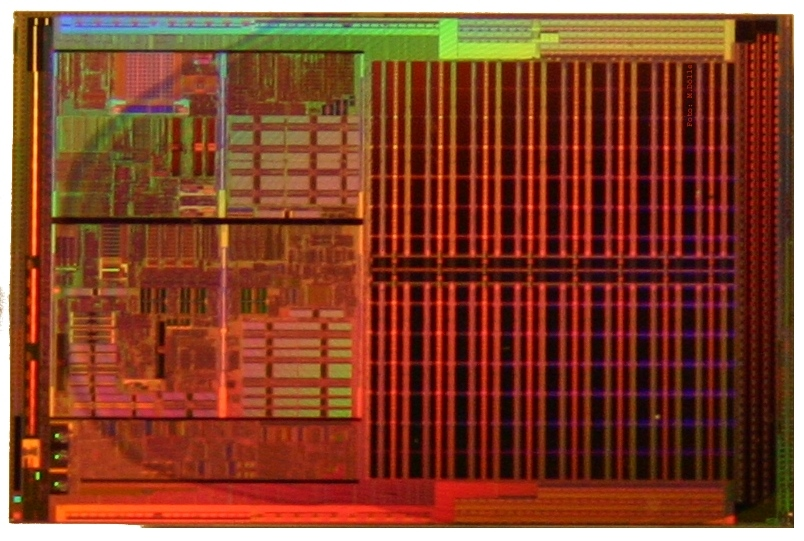
\includegraphics[width=3cm]{Opteron-die.jpg}};
\node[below=-2pt of cpu] {processor};
\node[anchor=center,right=8cm of cpu] (memory) {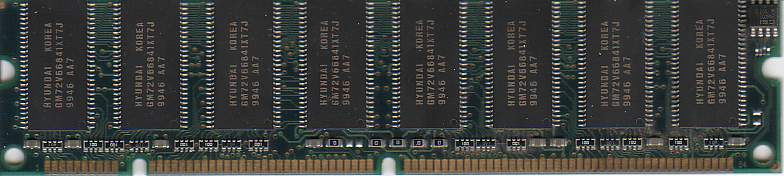
\includegraphics[height=0.75cm,angle=90]{SDRAM.jpg}};
\node[below=0pt of memory] {memory};

\onslide<1-3|handout:0>{
    \draw[latex-latex, line width=3pt] (cpu) -- (memory);
}
\coordinate (middleBus) at ($(cpu)!.5!(memory)$);


\onslide<3|handout:0>{
    \node[my callout2=middleBus,align=left] at ($(middleBus) + (-3cm,2cm)$) {memory bus \\ send address + send or get data};
}

\onslide<4->{
    \node[smallBox,anchor=center,fill=white, align=center] (ioBridge) at (middleBus) {I/O \\ Bridge};
    \draw[latex-latex, line width=3pt] (cpu) -- (ioBridge);
    \draw[latex-latex, line width=3pt] (ioBridge) -- (memory);
    \coordinate (toIO) at ($(middleBus) + (0,-3cm)$);
    \draw[latex-latex, line width=3pt] (ioBridge) -- (toIO);
    \node[below=0pt of toIO, align=left] {to I/O devices \\ \small keyboard, mouse, wifi, \ldots};
    \coordinate (middleSysBus) at ($(cpu)!.5!(middleBus)$);
    \coordinate (middleMemBus) at ($(memory)!.5!(middleBus)$);
    \coordinate (middleIOBus) at ($(middleBus)!.5!(toIO)$);
}
\onslide<5>{
    \node[my callout2=middleSysBus,align=left] at ($(middleSysBus) + (0,2cm)$) {system bus \\ send address + send or get data \\ (machine code/text/number\ldots)};
}
\onslide<6-7>{
    \node[my callout2=middleSysBus,align=left] at ($(middleSysBus) + (0,2cm)$) {CPU: send PC: {\tt 0x04000}};
    \node[my callout2=middleMemBus,align=left] at ($(middleMemBus) + (-3cm,-2cm)$) {MEM: send machine code:\\{\tt pushq \%rbp}};
}
\onslide<7>{
    \node[my callout2=middleSysBus,align=left] at ($(middleSysBus) + (0,1cm)$) {CPU: next PC: {\tt 0x04001}};
}
\onslide<8>{
    \node[my callout2=middleSysBus,align=left] at ($(middleSysBus) + (-2,2cm)$) {CPU: send I/O request address: {\tt 0xf122003}};
    \node[my callout2=middleIOBus,align=left] at ($(middleIOBus) + (1cm,0)$) {I/O: send keystoke: ``a''};
}
\end{tikzpicture}
\imagecredit{Images: \\
             Single core Opteron 8xx die: Dg2fer at the German language Wikipedia, via Wikimedia Commons \\
             SDRAM by Arnaud 25, via Wikimedia Commons}
\end{frame}


\newcommand{\memoryPicture}{
\matrix (memoryWithLabels) [matrix of nodes,
    row sep=2mm,
    inner sep=0mm,
    font=\small\ttfamily,
    nodes={text depth=0pt,inner sep=0.2mm,inner xsep=1mm},
    column 1/.style={align=right,column sep=2mm},
    column 2/.style={align=left,minimum width=1cm},
    row 1/.style={font=\small\bfseries}] {
        address \& value \\
        0xFFFFFFFF  \& 0x14\\
        0xFFFFFFFE  \& 0x45\\
        0xFFFFFFFD  \& 0xDE\\
        \ldots  \& \ldots \\
        0x00042006  \& 0x06\\
        0x00042005  \& 0x05\\
        0x00042004  \& 0x04\\
        0x00042003  \& 0x03\\
        0x00042002  \& 0x02\\
        0x00042001  \& 0x01\\
        0x00042000  \& 0x00\\
        0x00041FFF  \& 0x03\\
        0x00041FFE  \& 0x60\\
        \ldots  \& \ldots \\
        0x00000002  \& 0xFE\\
        0x00000001  \& 0xE0\\
        0x00000000  \& 0xA0\\
};
\draw[black!80!white,line width=1pt] (memoryWithLabels-2-2.north west) rectangle (memoryWithLabels-4-2.south east);
\draw[black!80!white,line width=1pt] (memoryWithLabels-6-2.north west) rectangle (memoryWithLabels-14-2.south east);
\draw[black!80!white,line width=1pt] (memoryWithLabels-16-2.north west) rectangle (memoryWithLabels-18-2.south east);
\foreach \x in {3,4,7,8,...,14,17,...,18} {
    \draw[black!80!white,line width=1pt] (memoryWithLabels-\x-2.north west) -- (memoryWithLabels-\x-2.north east);
}
}

\begin{frame}[fragile,label=endiannes]{endianness}
\begin{tikzpicture}
\memoryPicture
\node[right=10mm of memoryWithLabels-2-2] (code) {
\begin{minipage}{4cm}
\begin{minted}{c++}
int *x = (int*)0x42000;
cout << *x << endl;
\end{minted}
\end{minipage}
};
%\node[right=1mm of memoryWithLabels-12-2] {\Huge$\Leftarrow$};
\onslide<2->{
    \node[fit=(memoryWithLabels-9-2) (memoryWithLabels-12-2),rectangle,draw=orange!70!black,line width=1mm] {};
}
\onslide<3->{
    \node[below=.2cm of code,xshift=10mm] (le) {\ttfamily 0x030201\myemph{00} $=$};
    \node[right=0cm of le] (leDec) {50462976};
    \node[below=2cm of le] (be) {\ttfamily 0x\myemph{00}010203 $=$};
    \node[right=0cm of be] (beDec) {66051};
}
\begin{pgfonlayer}{bg}
\onslide<4->{
    \node[below=.1cm of le,xshift=.5cm,fill=blue!20, align=center] {little endian \\ (least significant byte has lowest address)};
    \node[fit=(leDec),inner sep=1mm,draw=blue!70!black,fill=blue!10, line width=1mm] (boxLe) {};
    \node[below=.1cm of be,xshift=.5cm,fill=green!20, align=center] {big endian \\ (most significant byte has lowest address)};
    \node[fit=(beDec),inner sep=1mm,draw=green!70!black,fill=green!10, line width=1mm] (boxBe) {};
}
\end{pgfonlayer}
\onslide<5->{
}
\end{tikzpicture}
\end{frame}


\begin{frame}[label=compPipe,fragile]{what's in those files?}
    \lstset{
        language=[x8664gas]Assembler,
        %moredelim=**[is][\color{green!60!black}]{@1*}{*@},
        moredelim=**[is][\cbA<5->]{@1*}{*@},
        moredelim=**[is][\cbB<5->]{@2*}{*@},
        moredelim=**[is][\cbC<5->]{@3*}{*@},
        moredelim=**[is][\cbD<5->]{@4*}{*@},
        escapechar=`,
    }
    \vspace{-.5cm}
    \begin{tikzpicture}
    \tikzset{
        mybox part/.style={minimum width=2cm,font=\scriptsize,align=left},
        mybox/.style={draw,rectangle,mybox part},
        mylabel/.style 2 args={label={[label distance=-1mm,inner sep=1mm,fill=white,draw,rectangle,font=\footnotesize,visible on=#2]90:#1}},
        myline/.style={line width=1pt,-latex},
    }
    \makeatletter
    \newenvironment{mycolorbox}[1]
    {\def\savedcolor{#1}\begin{lrbox}{\@tempboxa}\strut}
    {\end{lrbox}\setlength{\fboxsep}{0pt}\colorbox{\savedcolor}{\usebox{\@tempboxa}}}
    \makeatother
    \def\doEndEnv{\end{mycolorbox}\egroup}
    \newcommand<>{\cbA}{\only#1{\begin{mycolorbox}{blue!40!white}\bgroup\aftergroup\doEndEnv}}
    \newcommand<>{\cbB}{\only#1{\begin{mycolorbox}{green!30!white}\bgroup\aftergroup\doEndEnv}}
    \newcommand<>{\cbC}{\only#1{\begin{mycolorbox}{red!20!white}\bgroup\aftergroup\doEndEnv}}
    \newcommand<>{\cbD}{\only#1{\begin{mycolorbox}{orange!30!white}\bgroup\aftergroup\doEndEnv}}

    \node[mybox,mylabel={hello.c}{<1->}] (helloC){
        \begin{minipage}{4cm}
\begin{ccode*}{xleftmargin=0cm,linenos=false}
#include <stdio.h>
int main(void) {
  puts("Hello, World!");
  return 0;
}
\end{ccode*} 
        \end{minipage}
    };

    \node[mybox,mylabel={hello.s}{<2->},anchor=north west,visible on=<2->] (helloS) at ($(helloC.north east) + (2cm, 0)$) {
\begin{lstlisting}
    .text
main:
    @2*sub  $8, %rsp*@
    mov  $@1*.Lstr*@, %rdi
    call @3*puts*@
    xor  %eax, %eax
    add  $8, %rsp
    ret

    .data
@1*.Lstr*@: .string @4*"Hello, World!"*@
\end{lstlisting} 
    };

    \draw[myline,visible on=<2->] (helloC) -- (helloS);
    
    \node[mybox part,visible on=<3->,anchor=north west,inner sep=.5mm] (helloOText) at ($(helloC.south west) + (0, -1cm)$) {
        \textbf{text} (code) segment: \\
        \texttt{{\cbB<5->48 83 EC 08} BF {\cbA<5->00 00 00 00} E8 {\cbC<5->00 00}} \\
        \texttt{{\cbC<5->00 00} 31 C0 48 83 C4 08 C3}
    };
    \node[mybox part,visible on=<4->,anchor=north west,inner sep=.5mm] (helloOData) at (helloOText.south west) {
        \textbf{data} segment: \\
        \texttt{{\cbD<5->48 65 6C 6C 6F 2C 20 57 6F 72 6C 00}}
    };
    \node[mybox part,visible on=<6->,anchor=north west,inner sep=.5mm] (helloOReloc) at (helloOData.south west) {
        \textbf{relocations}: \\
        \begin{tabular}{ll}
        \it take 0s at & \it and replace with \\
        text, byte 6 ({\cbA$\;$}) & data segment, byte 0 \\
        text, byte 10 ({\cbC$\;$}) & address of \texttt{puts} \\
        \end{tabular}
    };
    \node[mybox part,visible on=<7->,anchor=north west,inner sep=.5mm] (helloOSymbols) at (helloOReloc.south west) {
        \textbf{symbol table}: \\
        \begin{tabular}{ll}
        \tt main & text byte 0 \\
        \end{tabular} 
    };
    \node[mybox,mylabel={hello.o}{<3->},anchor=north west,visible on=<3->,
          fit=(helloOText) (helloOSymbols),inner sep=0mm] (helloO) {};

    \draw[myline,visible on=<3->] (helloS) -- ($(helloO.north east) + (-1cm,0)$);

    \node[mybox,mylabel={hello.exe}{<8->},anchor=north west,visible on=<9->] (helloExe) at ($(helloS.south west) + (0, -1cm)$) {
        (actually binary, but shown as hexadecimal)
        \ldots \\
        \texttt{{\cbB 48 83 EC 08} BF {\cbA A7 02 04 00}} \\
        \texttt{E8 {\cbC 08 4A 04 00} 31 C0 48} \\
        \texttt{83 C4 08 C3} \ldots \\
        \ldots (code from stdio.o) \ldots \\
        \texttt{{\cbD 48 65 6C 6C 6F 2C 20 57 6F}} \\
        \texttt{{\cbD 72 6C 00}} \ldots \\
        \ldots (data from stdio.o) \ldots
    };

    \draw[myline,visible on=<8->] ($(helloO.east) + (0, 1cm)$) -- ($(helloExe.north) + (-1cm, 0)$) 
        node[midway,font=\footnotesize,rectangle,fill=white,draw,thin] {+ stdio.o};
    \end{tikzpicture}
\end{frame}


\begin{frame}[fragile,label=realHelloS]{hello.s}
\begin{Verbatim}
        .section        .rodata.str1.1,"aMS",@progbits,1
.LC0:
        .string "Hello, World!"
        .text
        .globl  main
main:
        subq    $8, %rsp
        movl    $.LC0, %edi
        call    puts
        movl    $0, %eax
        addq    $8, %rsp
        ret
\end{Verbatim}
\end{frame}

\begin{frame}[fragile,label=realHelloO]{hello.o}
\begin{Verbatim}
hello.o:     file format elf64-x86-64

SYMBOL TABLE:
0000000000000000 g     F .text  0000000000000018 main
0000000000000000         *UND*  0000000000000000 puts

RELOCATION RECORDS FOR [.text]:
OFFSET           TYPE              VALUE 
0000000000000005 R_X86_64_32       .rodata.str1.1
000000000000000a R_X86_64_PC32     puts-0x0000000000000004

Contents of section .text:
 0000 4883ec08 bf000000 00e80000 0000b800  H...............
 0010 00000048 83c408c3                    ...H....        
Contents of section .rodata.str1.1:
 0000 48656c6c 6f2c2057 6f726c64 2100      Hello, World!.  
\end{Verbatim}
\end{frame}


\begin{frame}[fragile]{pointer arithmetic}
\begin{tikzpicture}
    \tikzset{
        mybox part/.style={minimum width=2cm,font=\scriptsize,align=left,fill=black!10!white},
        mybox/.style={draw,rectangle,mybox part},
        mycodebox/.style={draw,rectangle,mybox part,fill=white},
        mylabel/.style 2 args={label={[label distance=-1mm,inner sep=1mm,fill=white,draw,rectangle,font=\footnotesize,visible on=#2]90:#1}},
        myline/.style={line width=1pt,-latex},
    }
    \matrix[matrix of nodes,
        mylabel={read-only data}{<1->},mybox,
        nodes={draw,rectangle,minimum width=0mm,minimum height=.5cm, inner sep=0mm,anchor=south,
               font=\tt\scriptsize},
        xshift=3cm,
        inner sep=0mm,outer sep=0mm,
    ] (data) {
        \sf\ldots\&\lstinline|'H'|\&\lstinline|'e'|\&\lstinline|'l'|\&%
        \lstinline|'l'|\&\lstinline|'o'|\&\lstinline|' '|\&%
        \lstinline|'W'|\&\lstinline|'o'|\&\lstinline|'r'|\&%
        \lstinline|'l'|\&\lstinline|'d'|\&\lstinline|'!'|\&%
        \lstinline|'\0'|\&\sf\ldots\\
    };
    \node[mybox,below=2cm of data-1-2] (ptr0) {\tt hello + 0};
    \node[below=0pt of ptr0,visible on=<2->] (ptr0ex) {\scriptsize\tt 0x4005C0};
    \draw[myline] (ptr0) -- (data-1-2);
    \node[mybox,right=2cm of ptr0] (ptr5) {\tt hello + 5};
    \draw[myline] (ptr5) -- (data-1-7);
    \node[below=0pt of ptr5,visible on=<2->] (ptr5ex) {\scriptsize\tt 0x4005C5};

    \node[below=0pt of ptr0ex,visible on=<2->,font=\scriptsize] (ptr0ex2) {
        \lstinline|*(hello + 0)| is \lstinline|'H'|
    };
    \node[below=0pt of ptr5ex,visible on=<2->,font=\scriptsize] (ptr5ex2) {
        \lstinline|*(hello + 5)| is \lstinline|' '|
    };

    \node[below=0pt of ptr0ex2,visible on=<3->,font=\scriptsize] (ptr0ex3) {
        \lstinline|hello[0]| is \lstinline|'H'|
    };
    \node[below=0pt of ptr5ex2,visible on=<3->,font=\scriptsize] (ptr5ex3) {
        \lstinline|hello[5]| is \lstinline|' '|
    };
\end{tikzpicture}
\end{frame}


\begin{frame}[fragile,label=listsB]{some lists}
\lstset{language=C,style=script}
\vspace{-.5cm}
\begin{tikzpicture}
% FIXME:
\tikzset{
    codeBox/.style={draw,anchor=north west}
}
\node[codeBox] (sentinelCode) at (0,0) {
\begin{minipage}{5.5cm}
\begin{ccodeT}
short sentinel = -9999;
short *x;
x = malloc(sizeof(short)*4);
x[3] = sentinel;
...
\end{ccodeT}
\end{minipage}
};
\node[right=1cm of sentinelCode,label={x},draw] (xSent) {~};
\matrix[
    right=1cm of xSent,
    tight matrix,
    nodes={text width=.7cm,align=center},
    row 1/.style={nodes={draw=none,font=\scriptsize\tt}}] (xSentArr) {
    x[0] \& x[1] \& x[2] \& x[3] \\
    $1$ \& $2$ \& $3$ \& |[fill=black!20,text width=1.5cm]| {$-9999$} \\
};
\draw[-Latex,thick] (xSent) -- (xSentArr);
\node[codeBox] (rangeCode) at ([yshift=-.2cm]sentinelCode.south west) {
\begin{minipage}{5.5cm}
\begin{ccodeT}
typedef struct range_t {
    unsigned int length;
    short *ptr;
} range;
range x;
x.length = 3;
x.ptr = malloc(sizeof(short)*3);
...
\end{ccodeT}
\end{minipage}
};
\matrix[right=.5cm of rangeCode,tight matrix,nodes={text width=1.5cm},
    row 1/.style={nodes={draw=none,font=\tt}}] (rangeData) {
    x \\
    len: 3 \\ ptr: \\
};
\matrix[right=1cm of rangeData-2-1,tight matrix,
    nodes={text width=.7cm,align=center}] (rangePtrData) { 1 \& 2 \& 3 \\ };
\draw[thick,-Latex] (rangeData-3-1) -- (rangePtrData);
\node[codeBox] (listsCode) at ([yshift=-.2cm]rangeCode.south west) {
\begin{minipage}{5.5cm}
\begin{ccodeT}
typedef struct node_t {
    short payload;
    list *next;
} node;
node *x;
x = malloc(sizeof(node_t));
...
\end{ccodeT}
\end{minipage}
};
\node[right=1cm of listsCode,label={x},draw] (xLists) {~};
\matrix[right=2cm of xLists,label={*x},tight matrix,nodes={text width=2.5cm}] (xVal) {
   payload: 1 \\
   ptr: \\
};
\draw[-Latex,thick] (xLists) -- (xVal-1-1);
\draw[-Latex,thick] (xVal-2-1.east) -- ++(.5cm,0cm);
\begin{visibleenv}<2->
\draw[blue,line width=.5mm] ([xshift=.5cm,yshift=1cm]xSent.east) coordinate (topLine)
        -- ([xshift=.5cm,yshift=-1cm]xSent.east) 
        -- ([xshift=.5cm,yshift=1cm]rangeData.east)
        -- ([xshift=.5cm,yshift=-1cm]rangeData.east)
        -- ([xshift=.5cm,yshift=1cm]xLists.east)
        -- ([xshift=.5cm,yshift=-1cm]xLists.east);
\node[overlay,blue,font=\small,anchor=north east,align=right] at ([yshift=.6cm]topLine) {$\leftarrow$ on stack\\or regs};
\node[blue,font=\small,anchor=north west] at ([yshift=.2cm]topLine) {on heap $\rightarrow$};
\end{visibleenv}
\end{tikzpicture}
\end{frame}


\begin{frame}{AT\&T syntax in one slide}
    \begin{itemize}
    \item destination \myemph{last}
    \item {\tt ()} means value \myemph{in memory}
    \item {\tt disp(base, index, scale)} same as \\ {\tt memory[disp + base + index * scale]}
        \begin{itemize}
        \item omit disp (defaults to {\tt 0})
        \item and/or omit base (defaults to {\tt 0})
        \item and/or scale (defualts to {\tt 1})
        \end{itemize}
    \item {\tt \$} means constant
    \item plain number/label means value in memory
    \end{itemize}
\end{frame}

\begin{frame}[fragile,label=att2e1]{AT\&T syntax example (1)}
\lstset{
    language=[x8664gas]Assembler,
    %moredelim=**[is][\color{green!60!black}]{@1*}{*@},
    moredelim=**[is][\btHL<1|handout:0>]{@1*}{*@},
    moredelim=**[is][\btHL<2|handout:0>]{@2*}{*@},
    moredelim={**[is][\btHL<2,4|handout:0>]{@24*}{*@}},
    moredelim=**[is][\btHL<3|handout:0>]{@3*}{*@},
    moredelim=**[is][\btHL<4|handout:0>]{@4*}{*@},
    moredelim=**[is][\btHL<5|handout:0>]{@5*}{*@},
    moredelim=**[is][\btHL<6|handout:0>]{@6*}{*@},
    escapechar=`,
}
\begin{lstlisting}
mov@5*q*@ @3*$42*@, @2*(*@@24*%rbx*@@2*)*@
// memory[rbx] <- 42
\end{lstlisting}
    \begin{itemize}
    \item \myemph<2>{destination last}
    \item {\tt ()}s represent value \myemph<2>{in memory}
    \item \myemph<3>{constants} start with {\tt \$}
    \item \myemph<4>{registers} start with {\tt \%}
    \item {\tt q} (`quad') indicates \myemph<5>{length} (8 bytes)
    \begin{itemize}\item {\tt l}: 4; {\tt w}: 2; {\tt b}: 1
                   \item sometimes can be omitted\end{itemize}
    \end{itemize}
\end{frame}



\newcommand{\xZF}{\ensuremath{\mathtt{ZF}}\xspace}
\newcommand{\xSF}{\ensuremath{\mathtt{SF}}\xspace}
\newcommand{\xOF}{\ensuremath{\mathtt{OF}}\xspace}
\newcommand{\xCF}{\ensuremath{\mathtt{CF}}\xspace}

\begin{frame}<5>[fragile,label=cc2B]{closer look: condition codes (2)}
\begin{lstlisting}[language=myasm,style=small]
  // 2**63 - 1
  movq $0x7FFFFFFFFFFFFFFF, %rax
  // 2**63 (unsigned); -2**63 (signed)
  movq $0x8000000000000000, %rbx
  cmpq %rax, %rbx
// result = %rbx - %rax
\end{lstlisting}
\begin{itemize}
\item as signed: $-2^{63} - \left(2^{63} - 1\right) = \xcancel{-2^{64} + 1}\;\;1$ (overflow)
\item as unsigned: $2^{63} - \left(2^{63} - 1\right) = 1$
\end{itemize}
\begin{tabular}{l@{\hspace{1cm}}l@{\hspace{1cm}}l}
$\xZF = 0$ (false) & not zero & rax and rbx not equal\\
\only<3->{$\xSF = 0$ (false)} & \only<3->{not negative} & \only<3->{rax $<=$ rbx (if correct)} \\
\only<4->{$\xOF = 1$ (true)} & \only<4->{overflow as signed} & \only<4->{incorrect for signed}\\
\only<5->{$\xCF = 0$ (false)} & \only<5->{no overflow as unsigned} & \only<5->{correct for unsigned}\\
\end{tabular}
\end{frame}

\begin{frame}<2>[fragile,label=ccEx3C]{closer look: condition codes (3)}
\begin{lstlisting}[language=myasm]
  movq  $-1, %rax
  addq  $-2, %rax
// result = -3
\end{lstlisting}
\begin{itemize}
\item as signed: $-1 + (-2) = -3$
\item as unsigned: $(2^{64} - 1) + (2^{64} - 2) = \xcancel{2^{65} - 3}\;\;2^{64}-3$ (overflow)
\end{itemize}
\begin{tabular}{l@{\hspace{1cm}}l@{\hspace{1cm}}l}
$\xZF = 0$ (false) & not zero & result not zero\\
\only<2->{$\xSF = 1$ (true)}  & \only<2->{negative} & \only<2->{result is negative} \\
\only<2->{$\xOF = 0$ (false)} & \only<2->{no overflow as signed} & \only<2->{correct for signed} \\
\only<2->{$\xCF = 1$ (true)} & \only<2->{overflow as unsigned} & \only<2->{incorrect for unsigned} \\
\end{tabular}
\end{frame}


\begin{frame}[fragile,label=compSw1]{compiling switches (1)}
\begin{ccodeNL*}{fontsize=\small}
switch (a) {
    case 1: ...; break;   
    case 2: ...; break;
    ...
    default: ...
}
\end{ccodeNL*}
\lstset{
    language=myasm,
    style=smaller,
    escapechar=`,
    morekeywords=decq,
}
\begin{lstlisting}
    // same as if statement?
    cmpq $1, %rax
    je code_for_1
    cmpq $2, %rax
    je code_for_2
    cmpq $3, %rax
    je code_for_3
    ...
    jmp code_for_default
\end{lstlisting}
\end{frame}

\begin{frame}[fragile,label=compSw2]{compiling switches (2)}
\begin{ccodeNL*}{fontsize=\small}
switch (a) {
    case 1: ...; break;
    case 2: ...; break;
    ...
    case 100: ...; break;
    default: ...
}
\end{ccodeNL*}
\lstset{
    language=myasm,
    style=smaller,
    escapechar=`,
    morekeywords=decq,
}
\begin{lstlisting}
    // binary search
    cmpq $50, %rax
    jl code_for_less_than_50
    cmpq $75, %rax
    jl code_for_50_to_75
    ...
code_for_less_than_50:
    cmpq $25, %rax
    jl less_than_25_cases
    ...
\end{lstlisting}
\end{frame}

\begin{frame}[fragile,label=compSw3]{compiling switches (3)}
\begin{ccodeNL*}{fontsize=\small}
switch (a) {
    case 1: ...; break;
    case 2: ...; break;
    ...
    case 100: ...; break;
    default: ...
}
\end{ccodeNL*}
\lstset{
    language=myasm,
    style=smaller,
    escapechar=`,
    morekeywords={decq,.quad}
}
\begin{tabular}{l@{\hspace{1cm}}l}
{\begin{lstlisting}
// jump table
cmpq $100, %rax
jg code_for_default
cmpq $1, %rax
jl code_for_default
jmp *table(,%rax,8)
\end{lstlisting}
}
    &
{\begin{lstlisting}
table:
  // not instructions
  // .quad = 64-bit (4 x 16) constant
  .quad code_for_1
  .quad code_for_2
  .quad code_for_3
  .quad code_for_4
    ...
\end{lstlisting}
} 
\end{tabular}
\end{frame}

\begin{frame}[fragile,label=computeJump]{computed jumps}
\lstset{
    language=myasm,
    morekeywords={decq,.quad}
}
\begin{lstlisting}[language=myasm]
  cmpq $100, %rax
  jg code_for_default
  cmpq $1, %rax
  jl code_for_default
  // jump to memory[table + rax * 8]
    // table of pointers to instructions
  jmp *table(,%rax,8)
  // intel: jmp QWORD PTR[rax*8 + table]
  ...
table:
  .quad code_for_1
  .quad code_for_2
  .quad code_for_3
  ...
\end{lstlisting}
\end{frame}



\begin{frame}[fragile,label=pushpop]{push/pop}
\begin{itemize}
    \item \lstinline|pushq %rbx|
    \begin{itemize}
        \item \lstinline|%rsp| $\leftarrow$ \lstinline|%rsp| $-\;8$
        \item memory[\lstinline|%rsp|] $\leftarrow$ \lstinline|%rbx|
    \end{itemize}
    \item \lstinline|popq %rbx|
    \begin{itemize}
        \item \lstinline|%rbx| $\leftarrow$ memory[\lstinline|%rsp|]
        \item \lstinline|%rsp| $\leftarrow$ \lstinline|%rsp| $+\;8$
    \end{itemize}
\end{itemize}
\begin{tikzpicture}[overlay,remember picture]
    \tikzset{offstack/.style={fill=black!25}}
    \matrix[matrix of nodes,row sep=-\pgflinewidth,
            nodes={font=\scriptsize,draw,rectangle,minimum width=4cm},
            above left=.5cm of current page.south east] (stack) {
            \vdots{} \\
        memory[\lstinline|%rsp| + 16] \\
        memory[\lstinline|%rsp| + 8] \\
        memory[\lstinline|%rsp|] \\
        |[offstack]| memory[\lstinline|%rsp| - 8] \\
        |[offstack]| memory[\lstinline|%rsp| - 16] \\
    };
    \node[left=1cm of stack-4-1,font=\small] (popMarker) {value to pop};
    \node[left=1cm of stack-5-1,font=\small] (pushMarker) {where to push};
    \draw[very thick] ([xshift=-1cm]stack-4-1.south west) -- ([xshift=1cm]stack-4-1.south east);
    %\draw[very thick,black!50,dotted] ([xshift=-1cm]stack-3-1.south west) -- ([xshift=1cm]stack-3-1.south east);
    %\draw[very thick,black!50,dotted] ([xshift=-1cm]stack-5-1.south west) -- ([xshift=1cm]stack-5-1.south east);
    \draw[-Latex,thick,double,black!60] ([xshift=-.2cm]stack-1-1.north west) -- ([xshift=-.2cm]stack-3-1.west)
        node[midway,left,align=right,font=\scriptsize]{stack\\growth};
    \draw[-Latex] (popMarker) -- (stack-4-1.west);
    \draw[-Latex] (pushMarker) -- (stack-5-1.west);
\end{tikzpicture}
\end{frame}


\begin{frame}[fragile,label=Y86format]{Y86-64 instruction formats}
\begin{tikzpicture}
\instrEncodingTable
\end{tikzpicture}
\end{frame}

\begin{frame}[fragile,label=Y86fn]{Secondary opcodes: {\keywordstyle {\it OP}q}}
\begin{tikzpicture}
\tikzset{extra box/.style={opacity=0.5},
         extra box fn/.style={opacity=1.0}}
\instrEncodingTable
\tikzset{
    hilite/.style={draw,rectangle,rounded corners,line width=2pt,red!80!black}
}
\node[fit=(table-8-3),hilite] (fnHi) {};
\node[yshift=1.5cm,right=0cm of table-8-5.north east,anchor=north west,opacity=.95,fill=white,draw,rectangle,draw=blue!30!black,line width=2pt] (fnTable) {
    \def\arraystretch{1.4}
    \begin{tabular}{ll}
    \fnify{0} & {\keywordstyle add} \\
    \fnify{1} & {\keywordstyle sub} \\
    \fnify{2} & {\keywordstyle and} \\ 
    \fnify{3} & {\keywordstyle xor} \\ 
    \end{tabular}
};
\end{tikzpicture}
\end{frame}

\begin{frame}[fragile,label=Y86reg]{Registers: \rA, \rB}
\begin{tikzpicture}
\tikzset{extra box/.style={opacity=0.6},
         extra box register/.style={opacity=1.0}}
\instrEncodingTable
\tikzset{
    hilite/.style={draw,rectangle,rounded corners,line width=2pt,red!80!black}
}
\node[hilite,fit=(table-4-4) (table-4-5) (table-8-4) (table-8-5)] {};
\node[hilite,fit=(table-12-4) (table-12-5) (table-13-4) (table-13-5)] {};
\node[yshift=1cm,right=1.25cm of table-2-3.north east,anchor=north west,opacity=.95,fill=white,draw,rectangle,draw=blue!30!black,line width=2pt] (fnTable) {
    \def\arraystretch{1.4}
    \tt
    \begin{tabular}{ll@{\hspace{1cm}}ll}
    \rnify{0} & \%rax & \rnify{8} & \%r8 \\
    \rnify{1} & \%rcx & \rnify{9} & \%r9 \\
    \rnify{2} & \%rdx & \rnify{A} & \%r10 \\ 
    \rnify{3} & \%rbx & \rnify{B} & \%r11 \\
    \rnify{4} & \%rsp & \rnify{C} & \%r12 \\
    \rnify{5} & \%rbp & \rnify{D} & \%r13 \\
    \rnify{6} & \%rsi & \rnify{E} & \%r14 \\
    \rnify{7} & \%rdi & \literalify{F} & \normalfont\it none\\
    \end{tabular}
};
\end{tikzpicture}
% FIXME: Why F in blank spots
% FIXME: Why rB not rA for irmovq
\end{frame}

\begin{frame}[fragile,label=Y86immed]{Immediates: \V, \D, \Dest}
\begin{tikzpicture}
\tikzset{
    extra box/.style={opacity=0.5},
    extra box immediate/.style={opacity=1.0},
    hilite/.style={draw,rectangle,rounded corners,line width=2pt,red!80!black},
}
\instrEncodingTable
\node[visible on=<1>,hilite,fit=(V-5) (D-6) (D-7)] {};
\node[visible on=<2>,hilite,fit=(Dest-9) (Dest-10)] {};
\end{tikzpicture}
\end{frame}



\begin{frame}[fragile,label=bitStrat]{bitwise strategies}
    \begin{itemize}
        \item use paper, find subproblems, etc.
        \item mask and shift 
            \begin{itemize}
                \item \lstinline+(x & 0xF0) >> 4+
            \end{itemize}
        \item factor/distribute
            \begin{itemize}
                \item \lstinline+(x & 1) | (y & 1) == (x | y) & 1+
            \end{itemize}
        \item divide and conquer
        \item common subexpression elimination
            \begin{itemize}
                \item \lstinline+return ((-!!x) & y) | ((-!x) & z)+
                \item becomes
                \item \lstinline+d = !x; return ((-!d) & y) | ((-d) & z)+
            \end{itemize}
    \end{itemize}
\end{frame}


\begin{frame}[fragile,label=shLwires]{shift left}
    \begin{itemize}
    \item x86 instruction: {\keywordstyle shl} --- shift left
    \item {{\keywordstyle shl} \tt\$\textit{amount}, \%reg} (or variable: {\tt{\keywordstyle shr} \%cl, \%reg})
    \end{itemize}
\begin{tikzpicture}
\draw[blue,decorate,decoration=brace,ultra thick] (-.2, .7) -- (13., .7) node[midway, above] {\%reg (initial value)};
\draw[blue,decorate,decoration={brace,mirror},ultra thick] (-.2, -3.1) -- (13., -3.1) node[midway, below] {\%reg (final value)};
\foreach \x/\v in {0/1,1/0,2/1,3/1} {
    \node[anchor=south] at ($(0,0) + \x*(0.4, 0)$) {\tt \v};
}
\foreach \x/\v in {4/0,5/0,6/1,7/\strut\ldots,27/\strut\ldots,28/0,29/1,30/0,31/0} {
    \node[anchor=south] at ($(0,0) + \x*(0.4, 0)$) {\tt \v};
    \node[anchor=north] at ($(0, -2.5) - 4*(0.4,0) + \x*(0.4, 0)$) {\tt \v};
}
\foreach \x in {4,5,6,7,...,31} {
    \draw[simple wire,->] ($(0,0) + \x*(0.4, 0)$) -- ($(0,-2.5) - 4*(0.4, 0) + \x*(0.4, 0)$);
}
\foreach \x in {28,29,30,31} {
    \draw[simple wire,->,alt=<2>{red}{black}] ($(.5, 0) + (0,-2) + \x*(0.4, 0)$) node[above] {\tt 0} -- ($(0,-2.5) + \x*(0.4, 0)$);
    \node[anchor=north,alt=<2>{red}{black}] at ($(0,-2.5) + \x*(0.4, 0)$) {\tt 0};
}
\end{tikzpicture}
\end{frame}

\begin{frame}[fragile,label=leftShift]{left shift in math}
% FIXME: 1s/2s/4s place diagram
\begin{tabular}{l@{\hspace{3cm}}l}
\lstinline|1 << 0 == 1| & \tt 0000 0001 \\
\lstinline|1 << 1 == 2| & \tt 0000 001\color{red!60}0 \\
\lstinline|1 << 2 == 4| & \tt 0000 01\color{red!60}00 \\
~ & ~ \\
\lstinline|10 << 0 == 10| & \tt 0000 1010 \\
\lstinline|10 << 1 == 20| & \tt 0001 010\color{red!60}0 \\
\lstinline|10 << 2 == 40| & \tt 0010 10\color{red!60}00 \\
\end{tabular}
\vspace{0.3cm}
\begin{center}
\begin{visibleenv}<2->
\large
$x$ \lstinline|<<| $y = x \times 2^y$
\end{visibleenv}
\end{center}
\end{frame}

\begin{frame}<1-3>[fragile,label=exposeWireSel]{logical right shift}
\begin{itemize}
\item x86 instruction: {\keywordstyle shr} --- logical shift right
\item {{\keywordstyle shr} \tt\$\textit{amount}, \%reg} (or variable: {\tt{\keywordstyle shr} \%cl, \%reg})
\end{itemize}
\begin{tikzpicture}
\draw[blue,decorate,decoration=brace,ultra thick] (-.2, .7) -- (13., .7) node[midway, above] {\%reg (initial value)};
\draw[blue,decorate,decoration={brace,mirror},ultra thick] (-.2, -3.1) -- (13., -3.1) node[midway, below] {\%reg (final value)};
\foreach \x/\v in {28/0,29/0,30/1,31/0} {
    \node[anchor=south] at ($(0,0) + \x*(0.4, 0)$) {\tt \v};
}
\foreach \x/\v in {0/0,1/0,2/0,3/\strut\ldots,23/\strut\ldots,24/0,25/1,26/1,27/1} {
    \node[anchor=south] at ($(0,0) + \x*(0.4, 0)$) (top-\x) {\tt \v};
    \node[anchor=north] at ($(0, -2.5) + 4*(0.4,0) + \x*(0.4, 0)$) (bottom-\x) {\tt \v};
}
\foreach \x in {0,1,2,3,...,27} {
    \draw[simple wire,->] ($(0,0) + \x*(0.4, 0)$) -- ($(0,-2.5) + 4*(0.4, 0) + \x*(0.4, 0)$);
}
\begin{visibleenv}<1>
    \node[draw,red,very thick,fit=(top-24) (top-27)] {};
    \node[draw,red,very thick,fit=(bottom-24) (bottom-27)] {};
\end{visibleenv}
\begin{visibleenv}<2>
\foreach \x in {0,1,2,3} {
    \node[anchor=north,red] at ($(0,-2.5) + \x*(0.4, 0)$) {\tt\bfseries ?};
}
\end{visibleenv}
\begin{visibleenv}<3-4>
\foreach \x in {0,1,2,3} {
    \draw[simple wire,->,alt=<2>{red}{black}] ($(-.5, 0) + (0,-2) + \x*(0.4, 0)$) node[above] {\tt 0} -- ($(0,-2.5) + \x*(0.4, 0)$);
    \node[anchor=north,alt=<2>{red}{black}] at ($(0,-2.5) + \x*(0.4, 0)$) {\tt 0};
}
\end{visibleenv}
\foreach \x in {28,29,30,31} {
    \fill[top color=black,bottom color=white] ($(0,0) + \x*(0.4, 0)$) rectangle ($(0,-0.5) + \x*(0.4, 0) + (.5pt, 0pt)$);
}
\end{tikzpicture}
\end{frame}

\begin{frame}{arithmetic right shift}
\begin{itemize}
\item x86 instruction: {\keywordstyle sar} --- arithmetic shift right
\item {{\keywordstyle sar} \tt\$\textit{amount}, \%reg} (or variable: {\tt{\keywordstyle sar} \%cl, \%reg})
\end{itemize}
\begin{tikzpicture}
\draw[blue,decorate,decoration=brace,ultra thick] (-.2, .7) -- (13., .7) node[midway, above] {\%reg (initial value)};
\draw[blue,decorate,decoration={brace,mirror},ultra thick] (-.2, -3.1) -- (13., -3.1) node[midway, below] {\%reg (final value)};
\foreach \x/\v in {28/1,29/0,30/1,31/1} {
    \node[anchor=south] at ($(0,0) + \x*(0.4, 0)$) {\tt \v};
}
\foreach \x/\v in {1/0,2/1,3/\strut\ldots,23/\strut\ldots,24/0,25/1,26/0,27/0} {
    \node[anchor=south] at ($(0,0) + \x*(0.4, 0)$) {\tt \v};
    \node[anchor=north] at ($(0, -2.5) + 4*(0.4,0) + \x*(0.4, 0)$) {\tt \v};
}
\foreach \x in {0,1,2,3,...,27} {
    \draw[simple wire,->] ($(0,0) + \x*(0.4, 0)$) -- ($(0,-2.5) + 4*(0.4, 0) + \x*(0.4, 0)$);
}
\begin{visibleenv}<1>
\foreach \x/\v in {0/0} {
    \node[blue,anchor=south] at ($(0,0) + \x*(0.4, 0)$) {\tt \v};
    \node[blue,anchor=north] at ($(0, -2.5) + 4*(0.4,0) + \x*(0.4, 0)$) {\tt \v};
}
\foreach \x in {0,1,2,3} {
    \draw[simple wire,->,blue] (0,0) -- ($(0,-2.5) + \x*(0.4, 0)$);
    \node[blue,anchor=north] at ($(0,-2.5) + \x*(0.4, 0)$) {\tt\bfseries 0};
}
\end{visibleenv}

\begin{visibleenv}<2>
\foreach \x/\v in {0/1} {
    \node[blue,anchor=south] at ($(0,0) + \x*(0.4, 0)$) {\tt \v};
    \node[blue,anchor=north] at ($(0, -2.5) + 4*(0.4,0) + \x*(0.4, 0)$) {\tt \v};
}
\foreach \x in {0,1,2,3} {
    \draw[simple wire,->,blue] (0,0) -- ($(0,-2.5) + \x*(0.4, 0)$);
    \node[blue,anchor=north] at ($(0,-2.5) + \x*(0.4, 0)$) {\tt\bfseries 1};
}
\end{visibleenv}
\end{tikzpicture}
\end{frame}

\begin{frame}[fragile,label=rightShiftC]{right shift in C}
\begin{ccodeNL}
int shift_signed(int x) {
    return x >> 5; // arithmetic; fill w/ copies of sign bit
}
unsigned shift_unsigned(unsigned x) {
    return x >> 5; // logical; fill with zeroes
}
\end{ccodeNL}
\hrule
\begin{tabular}{ll}
\begin{asmcodeNL}
shift_signed:
    movl %edi, %eax
    sarl $5, %eax
    ret
\end{asmcodeNL}
&
\begin{asmcodeNL}
shift_unsigned:
    movl %edi, %eax
    shrl $5, eax
    ret
\end{asmcodeNL}
\end{tabular}
\end{frame}



\usetikzlibrary{patterns,positioning}

\begin{frame}[fragile,label=SumRegisterOperation]{registers}
    \begin{tikzpicture}
        \node[hReg=PC] (pc) {};
        \draw[a,latex-] (pc.west) -- ++(-1cm, 0cm);
        \draw[a] (pc.east) -- ++(1cm, 0cm);
        \node[below=1.5cm of pc,visible on=<1>] (everyCC) {
            updates every \myemph{clock cycle}
        };
        \begin{scope}[shift={($(everyCC.east)+(1cm,-.5cm)$)}] 
            \draw[very thick] (0, 0) -- (1, 0) -- (1, 1) -- (2, 1) -- (2, 0) -- (3, 0) -- (3, 1) -- (4, 1);
            \draw[ultra thick,red!95!black] (1, 0) -- (1, 1);
            \draw[ultra thick,red!95!black] (3, 0) -- (3, 1);
        \end{scope}
        \begin{scope}[shift={($(everyCC.east)+(1cm,-.6cm)$)}] 
            \fill[color=blue!80!black] (0, 0) rectangle (0.99, -.5);
            \fill[color=green!40!white] (1.01, 0) rectangle (2.99, -.5);
            \fill[color=violet!60!black] (3.01, 0) rectangle (4., -.5);
            \node[anchor=east,font=\small] at (0,-.25) {register output};
            \fill[pattern=north west lines] (0.0, -0.6) rectangle (0.2, -1.1);
            \fill[color=green!40!white] (0.2, -0.6) rectangle (1.01, -1.1);
            \fill[pattern=north west lines] (1.01, -0.6) rectangle (1.7, -1.1);
            \fill[color=violet!60!black] (1.7, -0.6) rectangle (3.01, -1.1);
            \fill[pattern=north west lines] (3.01, -0.6) rectangle (3.9, -1.1);
            \fill[color=orange!40] (3.9, -0.6) rectangle (4., -1.1);
            \node[anchor=east,font=\small] at (0,-.85) {register input};
        \end{scope}
    \end{tikzpicture}
\end{frame}

\begin{frame}[fragile,label=SumY86stateOnly]{state in Y86-64}
    \begin{tikzpicture}
        \tikzset{
            imemPcPre/.style={visible on=<1-|handout:1>},
            regPre/.style={visible on=<0|handout:0>},
            regPreSingle/.style={visible on=<1-|handout:1>},
            imemPc/.style={visible on=<0|handout:0>},
            instrRegsPreSingle/.style={visible on=<1-|handout:1>},
            instrRegsPre/.style={visible on=<0|handout:0>},
            instrRegs/.style={visible on=<0|handout:0>},
            regsLogic/.style={visible on=<0|handout:0>},
            logicDmem/.style={visible on=<0|handout:0>},
            pcDecode/.style={visible on=<0|handout:0>},
            dmemPre/.style={visible on=<1-|handout:1>},
            dmemWB/.style={visible on=<0|handout:0>},
            dmemPC/.style={visible on=<0|handout:0>},
            hiOver/.style={opacity=0.2,fill=green},
            ccsNorm/.style={visible on=<1-|handout:1>},
        }
        \circuitLayout
        \begin{visibleenv}<2|handout:0>
            \node[draw,red,ultra thick,fit=(pc)] {};
        \end{visibleenv}
        \begin{visibleenv}<3|handout:0>
            \node[draw,red,ultra thick,fit=(imem)] {};
        \end{visibleenv}
        \begin{visibleenv}<4|handout:0>
            \node[draw,red,ultra thick,fit=(regs)] {};
        \end{visibleenv}
        \begin{visibleenv}<5|handout:0>
            \node[draw,red,ultra thick,fit=(dmem)] {};
        \end{visibleenv}
        \begin{visibleenv}<2|handout:0>
            \node[draw,red,ultra thick,fit=(ccs)] {};
        \end{visibleenv}
    \end{tikzpicture}
\end{frame}

\begin{frame}[fragile,label=SumMem]{memories}
    \begin{tikzpicture}
        \node[mem] (imem) {Instr. \\ Mem.};
        \coordinate (imemData) at (imem.east);
        \coordinate (imemAddr) at (imem.west);
        \draw[thick,-latex] (imemData) -- +(.5cm,0cm) node [font=\small,right] { data };
        \draw[thick,latex-] (imemAddr) -- +(-.3cm,0cm) node [font=\small,left] { address };
        \onslide<2->{
            \node[mem,right=6cm of imem] (dmem) {Data \\ Mem.};
            \coordinate (dmemInHigh) at ($(dmem.west) + (0cm,-.5cm)$);
            \coordinate (dmemInLow) at ($(dmem.west) + (0cm,.5cm)$);
            \coordinate (dmemDataOut) at (dmem.east);
            \coordinate (dmemWE) at ([xshift=-.2cm]dmem.south);
            \coordinate (dmemRE) at ([xshift=.2cm]dmem.south);
            \draw[thick,-latex] (dmemDataOut) -- +(.3cm,0cm) node[right,font=\small] {data output};
            \draw[thick,latex-] (dmemInHigh) -- +(-.3cm,0cm) node[left,font=\small] { address };
            \draw[thick,latex-] (dmemInLow) -- +(-.3cm,0cm) node[left,font=\small,align=right] { input \\ to write };

            \draw[thin,latex-] (dmemWE) |- +(-1cm,-.3cm) node[left,inner sep=.05mm,font=\small] { write enable? };
            \draw[thin,latex-] (dmemRE) |- +(1cm,-.9cm) node[right,inner sep=.05mm,font=\small] { read enable? };
        }
        \begin{scope}[shift={($(imem.south east) + (-1, -3)$)}] 
            \node[anchor=east,font=\small] at (0,-.25) {address input};
            \fill[color=red!80!black] (0.1, 0) rectangle (2.0, -.5);
            \fill[pattern=north west lines] (0.0, -.6) rectangle (0.9, -1.1);
            \fill[color=blue!80!black] (0.9, -.6) rectangle (2.0, -1.1);
            \node[anchor=east,font=\small] at (0,-.85) {data output};
            \draw[thin,-latex] (0.0, -1.3) -- (1.5, -1.3) node[right,font=\scriptsize] {time};
        \end{scope}

        \onslide<3->{
        \begin{scope}[shift={($(dmem.south east) + (-1, -2.9)$)}] 
            \draw[very thick] (0, 0) -- (1, 0) -- (1, 1) -- (2, 1) -- (2, 0) -- (2.3, 0);
            \draw[very thick,opacity=0.2] (2.3,0) -- (3,0) -- (3,1) --  (4,1);
            \draw[ultra thick,red!95!black] (1, 0) -- (1, 1);
        \end{scope}
        \begin{scope}[shift={($(dmem.south east) + (-1, -3)$)}] 
            \node[anchor=east,font=\small] at (0,-.25) {address input};
            \fill[color=orange!70!black] (0.1, 0) rectangle (1.03, -.5);
            \node[anchor=east,font=\small] at (0,-.85) {input to write};
            \fill[pattern=north west lines] (0.0, -0.6) rectangle (0.2, -1.1);
            \fill[color=green!60!white] (0.2, -.6) rectangle (1.02, -1.1);
            \node[anchor=east,font=\small] at (0,-1.45) {value in memory};
            \fill[color=blue!80!black] (0, -1.2) rectangle (0.99, -1.7);
            \fill[color=green!60!white] (1.0, -1.2) rectangle (2.3, -1.7);
        \end{scope}
        }
    \end{tikzpicture}
\end{frame}

\begin{frame}[fragile,label=SumY86RegFile]{register file}
    \begin{tikzpicture}
        \tikzset{
            readReg/.style={blue!50!black},
            writeReg/.style={green!50!black}
        }
        \node[regFile] (regs) {register file \\ \scriptsize \%rax, \%rdx, \ldots{}};
        \coordinate (regSelect1) at ($(regs.north west) - (0cm, .4cm)$);
        \coordinate (regSelect2) at ($(regs.north west) - (0cm, .8cm)$);
        \coordinate (regSelect3) at ($(regs.north west) - (0cm, 1.4cm)$);
        \coordinate (regSelect4) at ($(regs.north west) - (0cm, 1.8cm)$);
        \coordinate (regWriteIn1) at ($(regs.north west) - (0cm, 2.8cm)$);
        \coordinate (regWriteIn2) at ($(regs.north west) - (0cm, 3.2cm)$);
        \coordinate (regRead1) at ($(regs.north east) - (0cm, .4cm)$);
        \coordinate (regRead2) at ($(regs.north east) - (0cm, .8cm)$);
        \foreach \x in {regSelect1,regSelect2} {
            \draw[readReg,latex-] (\x) -- +(-.5cm,0cm);
        }
        \foreach \x in {regSelect3,regSelect4} {
            \draw[writeReg,latex-] (\x) -- +(-.5cm,0cm);
        }
        \foreach \x in {regRead1,regRead2} {
            \draw[readReg,thick,-latex] (\x) -- +(.5cm,0cm);
        }
        \node[readReg,ll,above right=2pt of regRead1,outer sep=1pt,inner sep=0pt] {reg values};
        \draw[writeReg,thick,latex-] (regWriteIn1) -- +(-.5cm,0cm);
        \draw[writeReg,thick,latex-] (regWriteIn2) -- +(-.5cm,0cm);
        \node[readReg,ll,above left=2pt of regSelect1,outer sep=1pt,inner sep=0pt] (regNumLabel) {read reg \#s};
        \node[writeReg,ll,above left=2pt of regSelect3,outer sep=1pt,inner sep=0pt] (regNumLabel) {write reg \#s};
        \node[writeReg,ll,above left=2pt of regWriteIn1,outer sep=1pt,inner sep=0pt,align=right] {data to write};

        \begin{visibleenv}<2>
            \draw[red,thick,latex-] (regSelect1) -- ++(-.5cm,0cm);
            \draw[red,thick,-latex] (regRead1) -- ++(.5cm,0cm);
        \end{visibleenv}
        \begin{visibleenv}<2->
            \begin{scope}[shift={($(regs.south east) + (-1, -0.5)$)}] 
                \node[anchor=east,font=\small,alt=<2>{red}] at (0,-.25) {register number input};
                \fill[color=red!80!black] (0.1, 0) rectangle (2.0, -.5);
                \fill[pattern=north west lines] (0.0, -.6) rectangle (0.9, -1.1);
                \fill[color=blue!80!black] (0.9, -.6) rectangle (2.0, -1.1);
                \node[anchor=east,font=\small,alt=<2>{red}] at (0,-.85) {register value output};
                \draw[thin,-latex] (0.0, -1.3) -- (1.5, -1.3) node[right,font=\scriptsize] {time};
            \end{scope}
        \end{visibleenv}

        \begin{visibleenv}<3>
            \draw[red,thick,latex-] (regSelect3) -- ++(-.5cm,0cm);
            \draw[red,thick,latex-] (regWriteIn1) -- ++(-.5cm,0cm);
        \end{visibleenv}

        \begin{visibleenv}<3->
        \begin{scope}[shift={($(regs.south east) + (6, -0.4)$)}] 
            \draw[very thick] (0, 0) -- (1, 0) -- (1, 1) -- (2, 1) -- (2, 0) -- (2.3, 0);
            \draw[very thick,opacity=0.2] (2.3,0) -- (3,0) -- (3,1) --  (4,1);
            \draw[ultra thick,red!95!black] (1, 0) -- (1, 1);
        \end{scope}
        \begin{scope}[shift={($(regs.south east) + (6, -0.5)$)}] 
            \node[anchor=east,font=\small,alt=<3>{red}] at (0,-.25) {register number input};
            \fill[color=orange!70!black] (0.1, 0) rectangle (1.03, -.5);
            \node[anchor=east,font=\small,alt=<3>{red}] at (0,-.85) {data input};
            \fill[pattern=north west lines] (0.0, -0.6) rectangle (0.2, -1.1);
            \fill[color=green!60!white] (0.2, -.6) rectangle (1.02, -1.1);
            \node[anchor=east,font=\small] at (0,-1.45) {value in register};
            \fill[color=blue!80!black] (0, -1.2) rectangle (0.99, -1.7);
            \fill[color=green!60!white] (1.0, -1.2) rectangle (2.3, -1.7);
        \end{scope}
        \end{visibleenv}
        
        \begin{visibleenv}<4->
            \node[align=left] at ([xshift=4cm]regs.east) {
                write register \#15: write is ignored \\
                read register \#15: value is always 0
            };
        \end{visibleenv}
    \end{tikzpicture}
\end{frame}

\begin{frame}[fragile,label=SumALUs]{ALUs}
    \tikzset{alu/.style={trapezium,
            trapezium angle=30,
            shape border rotate=270,
            minimum width=4cm,
            minimum height=3cm,
            trapezium stretches=true,
            append after command={%
                    \pgfextra
                        \draw (\tikzlastnode.top left corner) --
                           (\tikzlastnode.top right corner) -- 
                           (\tikzlastnode.bottom right corner) -- 
                           ($(\tikzlastnode.bottom right corner)!.666!(\tikzlastnode.bottom side)$)--
                           ([xshift=8mm]\tikzlastnode.bottom side)--
                           ($(\tikzlastnode.bottom side)!.334!(\tikzlastnode.bottom left corner)$)--
                           (\tikzlastnode.bottom left corner)--
                           (\tikzlastnode.top left corner);
                    \endpgfextra}}}
    \begin{tikzpicture}
        \node[alu] (alu) {ALU};
        \draw[a] (alu.east) -- ++(0:5mm) node[right] (outLabel) {{\color{blue}A} {\it OP} {\color{green}B}};
        \draw[a,latex-] (alu.130) -- ++(180:5mm) node[left] {\color{blue} A};
        \draw[a,latex-] (alu.230) -- ++(180:5mm) node[left] {\color{green} B};
        \draw[b,latex-] (alu.south) -- ++(-90:2cm) node[below] {operation select};
        \node[draw, rectangle,below right=1cm and .2cm of outLabel, align=left] {
            Operations needed: \\
            add --- \addq, addresses \\
            sub --- \subq \\
            xor --- \xorq \\
            and --- \andq \\
            more?
        };
    \end{tikzpicture}
\end{frame}



\begin{frame}[fragile,label=pcUpdateCircuit]{SEQ circuit}
    \begin{tikzpicture}[circuit logic]
    \tikzset{
        dmemLabel/.style={visible on=<0|handout:0>},
        dmemInputLabel/.style={visible on=<1-|handout:1>},
        instrRegs/.style={visible on=<0|handout:0>},
        regsLogic/.style={visible on=<1-|handout:1>},
        regsLogicMux/.style={visible on=<0|handout:0>},
        regsLogicMuxA/.style={visible on=<1-|handout:1>},
        regsLogicNoMuxB/.style={visible on=<1-|handout:1>},
        logicDmem/.style={visible on=<1-|handout:1>},
        dmemPC/.style={visible on=<1-|handout:1>},
        dmemWB/.style={visible on=<1-|handout:1->},
        dmemOutToPC/.style={visible on=<1-|handout:1->},
        instrRegs/.style={visible on=<1-|handout:1>},
        %instrRegsSplitImmed/.style={visible on=<1-|handout:1>},
        instrRegsRS1/.style={visible on=<1-|handout:1>},
        instrRegsMux/.style={visible on=<1-|handout:1>},
    }
    \circuitState
    \circuitConnectDetail
    \draw[a] (iLenPlus) -- ++ (-1cm, 0cm) node[left,bookLabel] {valP};
    \end{tikzpicture}
\end{frame}



\begin{frame}<1-3|handout:1>[fragile,label=SettingMuxes]{circuit: setting MUXes}
\begin{tikzpicture}[circuit logic]
    \tikzset{
        dmemLabel/.style={visible on=<0|handout:0>},
        isStatReg/.style={draw=none},
        isStat/.style={draw=none},
        ccsNorm/.style={visible on=<0|handout:0>},
        hiBox/.style={fill=green,opacity=0.3},
        overText/.style={red,fill=white,fill opacity=0.7},
    }
    \circuitState
    \circuitConnectDetail
    \begin{visibleenv}<2-4>
    \begin{scope}[overlay]
        \node[overText,right=3pt of vrALabel,inner sep=0pt, outer sep=0pt, font=\tiny]{\tt 8}; 
        \node[overText,right=3pt of vrBLabel,inner sep=0pt, outer sep=0pt,font=\tiny]{\tt 9};
        \node[overText,below left=1cm and -.5cm of muxPc,font=\scriptsize,fill=white] {PC+2};
        \node[overText,above left=0.7cm and -1cm of muxPc,font=\scriptsize] {M[PC+1]};
        \node[overText,left=1pt of muxDstM.input 1,inner sep=0pt, outer sep=0pt,font=\tiny,yshift=.4ex]{rA=\tt 8};
        \node[overText,left=1pt of muxDstE.input 1,inner sep=0pt, outer sep=0pt,font=\tiny,yshift=.4ex]{rB=\tt 9};
        \node[overText,above right=0pt of regRead1,inner sep=0pt, outer sep=0pt,font=\tiny]{\tt R[8]};
        \node[overText,left=0.0cm of muxAluB.input 1,inner sep=0pt, outer sep=0pt,font=\tiny,yshift=.3ex]{\tt R[9]};
        \coordinate (eLabelPt) at ([yshift=-.25cm,xshift=1.25cm]regs.south east);
        \node[overText,inner sep=0pt, outer sep=0pt,font=\tiny,yshift=.4ex] at (eLabelPt) {\tt aluA + aluB};
        \coordinate (cLabel) at ([xshift=-2.5mm,yshift=2.15cm]muxAluA.input 1);
        \node[overText,inner sep=0pt, outer sep=0pt, font=\tiny,anchor=east] at (cLabel) {M[PC+2]};
        \draw (alu.south) -- ++(0,-2.5mm) node[below,inner sep=3pt,align=center,font=\scriptsize,fill=white,line width=2pt, draw=red,rectangle] (aluOverride) {add};
    \end{scope}
    \end{visibleenv}
    \begin{visibleenv}<1-4|handout:1>
    \begin{scope}[overlay]
        \node[draw,rectangle,line width=2pt,below right=1.8cm and -1.45cm of pc,text width=12cm,font=\small] {
            MUXes --- PC, dstM, dstE, aluA, aluB, dmemIn, dmemAddr, \ldots \\
            Exercise: what do they select when running \lstinline|addq %r8, %r9|?
        };
    \end{scope}
    \end{visibleenv}
    \begin{visibleenv}<3|handout:1>
        \draw[red,b] (muxSrcB.input 1) -- (muxSrcB.output);
        \draw[red,b] (muxDstM.input 2) -- (muxDstM.output);
        \draw[red,b] (muxDstE.input 1) -- (muxDstE.output);
        \draw[red,aa] (muxPc.input 3) -- (muxPc.output);
        \draw[red,aa] (muxAluA.input 2) -- (muxAluA.output);
        \draw[red,aa] (muxAluB.input 1) -- (muxAluB.output);
    \end{visibleenv}

    \begin{visibleenv}<5-6|handout:2>
    \begin{scope}[overlay]
        \node[draw,rectangle,line width=2pt,below right=1.8cm and -1.45cm of pc,text width=12cm,font=\small] {
            MUXes --- PC, dstM, dstE, aluA, aluB, dmemIn, dmemAddr, \ldots \\
            Exercise: what do they select for \rmmovq?
        };
    \end{scope}
    \end{visibleenv}
    \begin{visibleenv}<6|handout:2>
        \draw[red,b] (muxSrcB.input 1) -- (muxSrcB.output);
        \draw[red,b] (muxDstM.input 2) -- (muxDstM.output);
        \draw[red,b] (muxDstE.input 2) -- (muxDstE.output);
        \draw[red,aa] (muxPc.input 3) -- (muxPc.output);
        \draw[red,aa] (muxAluA.input 1) -- (muxAluA.output);
        \draw[red,aa] (muxAluB.input 1) -- (muxAluB.output);
    \end{visibleenv}
    \begin{visibleenv}<7|handout:3>
    \begin{scope}[overlay]
        \node[draw,rectangle,line width=2pt,below right=1.8cm and -1.45cm of pc,text width=12cm,font=\small] {
            MUXes --- PC, dstM, dstE, aluA, aluB, dmemIn, dmemAddr, \ldots \\
            Exercise: what do they select for {\keywordstyle irmovq}?
        };
    \end{scope}
    \end{visibleenv}

    \begin{visibleenv}<8|handout:4>
    \begin{scope}[overlay]
        \node[draw,rectangle,line width=2pt,below right=1.8cm and -1.45cm of pc,text width=12cm,font=\small] {
            MUXes --- PC, dstM, dstE, aluA, aluB, dmemIn, dmemAddr, \ldots \\
            Exercise: what do they select for {\keywordstyle mrmovq}?
        };
    \end{scope}
    \end{visibleenv}

    \begin{visibleenv}<9|handout:5>
    \begin{scope}[overlay]
        \node[draw,rectangle,line width=2pt,below right=1.8cm and -1.45cm of pc,text width=12cm,font=\small] {
            MUXes --- PC, dstM, dstE, aluA, aluB, dmemIn, dmemAddr, \ldots \\
            Exercise: what do they select for {\keywordstyle jle}?
        };
    \end{scope}
    \end{visibleenv}

    \begin{visibleenv}<10|handout:6>
    \begin{scope}[overlay]
        \node[draw,rectangle,line width=2pt,below right=1.8cm and -1.45cm of pc,text width=12cm,font=\small] {
            MUXes --- PC, dstM, dstE, aluA, aluB, dmemIn, dmemAddr, \ldots \\
            Exercise: what do they select for {\keywordstyle cmovle}?
        };
    \end{scope}
    \end{visibleenv}

    \begin{visibleenv}<11|handout:7>
    \begin{scope}[overlay]
        \node[draw,rectangle,line width=2pt,below right=1.8cm and -1.45cm of pc,text width=12cm,font=\small] {
            MUXes --- PC, dstM, dstE, aluA, aluB, dmemIn, dmemAddr, \ldots \\
            Exercise: what do they select for {\keywordstyle ret}?
        };
    \end{scope}
    \end{visibleenv}

    \begin{visibleenv}<12|handout:8>
    \begin{scope}[overlay]
        \node[draw,rectangle,line width=2pt,below right=1.8cm and -1.45cm of pc,text width=12cm,font=\small] {
            MUXes --- PC, dstM, dstE, aluA, aluB, dmemIn, dmemAddr, \ldots \\
            Exercise: what do they select for {\keywordstyle popq}?
        };
    \end{scope}
    \end{visibleenv}

    \begin{visibleenv}<13|handout:9>
    \begin{scope}[overlay]
        \node[draw,rectangle,line width=2pt,below right=1.8cm and -1.45cm of pc,text width=12cm,font=\small] {
            MUXes --- PC, dstM, dstE, aluA, aluB, dmemIn, dmemAddr, \ldots \\
            Exercise: what do they select for {\keywordstyle call}?
        };
    \end{scope}
    \end{visibleenv}
\end{tikzpicture}
\end{frame}

\againframe<5-6|handout:2>{SettingMuxes}

\againframe<7|handout:3>{SettingMuxes}

\againframe<8|handout:4>{SettingMuxes}

\againframe<9|handout:5>{SettingMuxes}

\againframe<10|handout:6>{SettingMuxes}

\againframe<11|handout:7>{SettingMuxes}

\againframe<12|handout:8>{SettingMuxes}

\againframe<13|handout:8>{SettingMuxes}


